\documentclass[twoside]{book}

% Packages required by doxygen
\usepackage{fixltx2e}
\usepackage{calc}
\usepackage{doxygen}
\usepackage[export]{adjustbox} % also loads graphicx
\usepackage{graphicx}
\usepackage[utf8]{inputenc}
\usepackage{makeidx}
\usepackage{multicol}
\usepackage{multirow}
\PassOptionsToPackage{warn}{textcomp}
\usepackage{textcomp}
\usepackage[nointegrals]{wasysym}
\usepackage[table]{xcolor}

% Font selection
\usepackage[T1]{fontenc}
\usepackage[scaled=.90]{helvet}
\usepackage{courier}
\usepackage{amssymb}
\usepackage{sectsty}
\renewcommand{\familydefault}{\sfdefault}
\allsectionsfont{%
  \fontseries{bc}\selectfont%
  \color{darkgray}%
}
\renewcommand{\DoxyLabelFont}{%
  \fontseries{bc}\selectfont%
  \color{darkgray}%
}
\newcommand{\+}{\discretionary{\mbox{\scriptsize$\hookleftarrow$}}{}{}}

% Page & text layout
\usepackage{geometry}
\geometry{%
  a4paper,%
  top=2.5cm,%
  bottom=2.5cm,%
  left=2.5cm,%
  right=2.5cm%
}
\tolerance=750
\hfuzz=15pt
\hbadness=750
\setlength{\emergencystretch}{15pt}
\setlength{\parindent}{0cm}
\setlength{\parskip}{3ex plus 2ex minus 2ex}
\makeatletter
\renewcommand{\paragraph}{%
  \@startsection{paragraph}{4}{0ex}{-1.0ex}{1.0ex}{%
    \normalfont\normalsize\bfseries\SS@parafont%
  }%
}
\renewcommand{\subparagraph}{%
  \@startsection{subparagraph}{5}{0ex}{-1.0ex}{1.0ex}{%
    \normalfont\normalsize\bfseries\SS@subparafont%
  }%
}
\makeatother

% Headers & footers
\usepackage{fancyhdr}
\pagestyle{fancyplain}
\fancyhead[LE]{\fancyplain{}{\bfseries\thepage}}
\fancyhead[CE]{\fancyplain{}{}}
\fancyhead[RE]{\fancyplain{}{\bfseries\leftmark}}
\fancyhead[LO]{\fancyplain{}{\bfseries\rightmark}}
\fancyhead[CO]{\fancyplain{}{}}
\fancyhead[RO]{\fancyplain{}{\bfseries\thepage}}
\fancyfoot[LE]{\fancyplain{}{}}
\fancyfoot[CE]{\fancyplain{}{}}
\fancyfoot[RE]{\fancyplain{}{\bfseries\scriptsize Generated by Doxygen }}
\fancyfoot[LO]{\fancyplain{}{\bfseries\scriptsize Generated by Doxygen }}
\fancyfoot[CO]{\fancyplain{}{}}
\fancyfoot[RO]{\fancyplain{}{}}
\renewcommand{\footrulewidth}{0.4pt}
\renewcommand{\chaptermark}[1]{%
  \markboth{#1}{}%
}
\renewcommand{\sectionmark}[1]{%
  \markright{\thesection\ #1}%
}

% Indices & bibliography
\usepackage{natbib}
\usepackage[titles]{tocloft}
\setcounter{tocdepth}{3}
\setcounter{secnumdepth}{5}
\makeindex

% Hyperlinks (required, but should be loaded last)
\usepackage{ifpdf}
\ifpdf
  \usepackage[pdftex,pagebackref=true]{hyperref}
\else
  \usepackage[ps2pdf,pagebackref=true]{hyperref}
\fi
\hypersetup{%
  colorlinks=true,%
  linkcolor=blue,%
  citecolor=blue,%
  unicode%
}

% Custom commands
\newcommand{\clearemptydoublepage}{%
  \newpage{\pagestyle{empty}\cleardoublepage}%
}

\usepackage{caption}
\captionsetup{labelsep=space,justification=centering,font={bf},singlelinecheck=off,skip=4pt,position=top}

%===== C O N T E N T S =====

\begin{document}

% Titlepage & ToC
\hypersetup{pageanchor=false,
             bookmarksnumbered=true,
             pdfencoding=unicode
            }
\pagenumbering{alph}
\begin{titlepage}
\vspace*{7cm}
\begin{center}%
{\Large A\+H\+RS }\\
\vspace*{1cm}
{\large Generated by Doxygen 1.8.13}\\
\end{center}
\end{titlepage}
\clearemptydoublepage
\pagenumbering{roman}
\tableofcontents
\clearemptydoublepage
\pagenumbering{arabic}
\hypersetup{pageanchor=true}

%--- Begin generated contents ---
\chapter{Data Structure Index}
\section{Data Structures}
Here are the data structures with brief descriptions\+:\begin{DoxyCompactList}
\item\contentsline{section}{\hyperlink{structmatrix}{matrix} }{\pageref{structmatrix}}{}
\item\contentsline{section}{\hyperlink{structvector}{vector} }{\pageref{structvector}}{}
\end{DoxyCompactList}

\chapter{File Index}
\section{File List}
Here is a list of all files with brief descriptions\+:\begin{DoxyCompactList}
\item\contentsline{section}{src/\hyperlink{BLASxOFF_8h}{B\+L\+A\+Sx\+O\+F\+F.\+h} }{\pageref{BLASxOFF_8h}}{}
\item\contentsline{section}{src/\hyperlink{copy__BLAS_8h}{copy\+\_\+\+B\+L\+A\+S.\+h} }{\pageref{copy__BLAS_8h}}{}
\item\contentsline{section}{src/gnd/inc/\hyperlink{BLAS__datatypes_8h}{B\+L\+A\+S\+\_\+datatypes.\+h} }{\pageref{BLAS__datatypes_8h}}{}
\item\contentsline{section}{src/gnd/inc/\hyperlink{matrix_8h}{matrix.\+h} }{\pageref{matrix_8h}}{}
\item\contentsline{section}{src/gnd/inc/\hyperlink{vector_8h}{vector.\+h} }{\pageref{vector_8h}}{}
\item\contentsline{section}{src/gnd/inc/\hyperlink{gnd_2inc_2vinit_8h}{vinit.\+h} }{\pageref{gnd_2inc_2vinit_8h}}{}
\item\contentsline{section}{src/gnd/src/\hyperlink{matrix_8c}{matrix.\+c} }{\pageref{matrix_8c}}{}
\item\contentsline{section}{src/gnd/src/\hyperlink{vector_8c}{vector.\+c} }{\pageref{vector_8c}}{}
\item\contentsline{section}{src/gnd/src/\hyperlink{gnd_2src_2vinit_8c}{vinit.\+c} }{\pageref{gnd_2src_2vinit_8c}}{}
\item\contentsline{section}{src/lvl0/inc/\hyperlink{array__add_8h}{array\+\_\+add.\+h} }{\pageref{array__add_8h}}{}
\item\contentsline{section}{src/lvl0/inc/\hyperlink{array__ascl_8h}{array\+\_\+ascl.\+h} }{\pageref{array__ascl_8h}}{}
\item\contentsline{section}{src/lvl0/inc/\hyperlink{array__asum_8h}{array\+\_\+asum.\+h} }{\pageref{array__asum_8h}}{}
\item\contentsline{section}{src/lvl0/inc/\hyperlink{array__copy_8h}{array\+\_\+copy.\+h} }{\pageref{array__copy_8h}}{}
\item\contentsline{section}{src/lvl0/inc/\hyperlink{array__dot_8h}{array\+\_\+dot.\+h} }{\pageref{array__dot_8h}}{}
\item\contentsline{section}{src/lvl0/inc/\hyperlink{array__mscl_8h}{array\+\_\+mscl.\+h} }{\pageref{array__mscl_8h}}{}
\item\contentsline{section}{src/lvl0/inc/\hyperlink{array__mult_8h}{array\+\_\+mult.\+h} }{\pageref{array__mult_8h}}{}
\item\contentsline{section}{src/lvl0/inc/\hyperlink{array__print_8h}{array\+\_\+print.\+h} }{\pageref{array__print_8h}}{}
\item\contentsline{section}{src/lvl0/inc/\hyperlink{array__puts_8h}{array\+\_\+puts.\+h} }{\pageref{array__puts_8h}}{}
\item\contentsline{section}{src/lvl0/inc/\hyperlink{array__set_8h}{array\+\_\+set.\+h} }{\pageref{array__set_8h}}{}
\item\contentsline{section}{src/lvl0/inc/\hyperlink{array__subtract_8h}{array\+\_\+subtract.\+h} }{\pageref{array__subtract_8h}}{}
\item\contentsline{section}{src/lvl0/inc/\hyperlink{array__swap_8h}{array\+\_\+swap.\+h} }{\pageref{array__swap_8h}}{}
\item\contentsline{section}{src/lvl0/inc/\hyperlink{array__zero_8h}{array\+\_\+zero.\+h} }{\pageref{array__zero_8h}}{}
\item\contentsline{section}{src/lvl0/inc/\hyperlink{level0_8h}{level0.\+h} }{\pageref{level0_8h}}{}
\item\contentsline{section}{src/lvl1/inc/\hyperlink{level1_8h}{level1.\+h} }{\pageref{level1_8h}}{}
\item\contentsline{section}{src/lvl1/inc/\hyperlink{vascl_8h}{vascl.\+h} }{\pageref{vascl_8h}}{}
\item\contentsline{section}{src/lvl1/inc/\hyperlink{vasum_8h}{vasum.\+h} }{\pageref{vasum_8h}}{}
\item\contentsline{section}{src/lvl1/inc/\hyperlink{vaxpy_8h}{vaxpy.\+h} }{\pageref{vaxpy_8h}}{}
\item\contentsline{section}{src/lvl1/inc/\hyperlink{vaxsy_8h}{vaxsy.\+h} }{\pageref{vaxsy_8h}}{}
\item\contentsline{section}{src/lvl1/inc/\hyperlink{vcopy_8h}{vcopy.\+h} }{\pageref{vcopy_8h}}{}
\item\contentsline{section}{src/lvl1/inc/\hyperlink{vcros3_8h}{vcros3.\+h} }{\pageref{vcros3_8h}}{}
\item\contentsline{section}{src/lvl1/inc/\hyperlink{vdot_8h}{vdot.\+h} }{\pageref{vdot_8h}}{}
\item\contentsline{section}{src/lvl1/inc/\hyperlink{vecld_8h}{vecld.\+h} }{\pageref{vecld_8h}}{}
\item\contentsline{section}{src/lvl1/inc/\hyperlink{lvl1_2inc_2vinit_8h}{vinit.\+h} }{\pageref{lvl1_2inc_2vinit_8h}}{}
\item\contentsline{section}{src/lvl1/inc/\hyperlink{vload_8h}{vload.\+h} }{\pageref{vload_8h}}{}
\item\contentsline{section}{src/lvl1/inc/\hyperlink{vmscl_8h}{vmscl.\+h} }{\pageref{vmscl_8h}}{}
\item\contentsline{section}{src/lvl1/inc/\hyperlink{vmult_8h}{vmult.\+h} }{\pageref{vmult_8h}}{}
\item\contentsline{section}{src/lvl1/inc/\hyperlink{vnrm1_8h}{vnrm1.\+h} }{\pageref{vnrm1_8h}}{}
\item\contentsline{section}{src/lvl1/inc/\hyperlink{vnrm2_8h}{vnrm2.\+h} }{\pageref{vnrm2_8h}}{}
\item\contentsline{section}{src/lvl1/inc/\hyperlink{vprint_8h}{vprint.\+h} }{\pageref{vprint_8h}}{}
\item\contentsline{section}{src/lvl1/inc/\hyperlink{vputs_8h}{vputs.\+h} }{\pageref{vputs_8h}}{}
\item\contentsline{section}{src/lvl1/inc/\hyperlink{vswap_8h}{vswap.\+h} }{\pageref{vswap_8h}}{}
\item\contentsline{section}{src/lvl1/inc/\hyperlink{vzero_8h}{vzero.\+h} }{\pageref{vzero_8h}}{}
\item\contentsline{section}{src/lvl1/src/\hyperlink{vascl_8c}{vascl.\+c} }{\pageref{vascl_8c}}{}
\item\contentsline{section}{src/lvl1/src/\hyperlink{vasum_8c}{vasum.\+c} }{\pageref{vasum_8c}}{}
\item\contentsline{section}{src/lvl1/src/\hyperlink{vaxpy_8c}{vaxpy.\+c} }{\pageref{vaxpy_8c}}{}
\item\contentsline{section}{src/lvl1/src/\hyperlink{vaxsy_8c}{vaxsy.\+c} }{\pageref{vaxsy_8c}}{}
\item\contentsline{section}{src/lvl1/src/\hyperlink{vcopy_8c}{vcopy.\+c} }{\pageref{vcopy_8c}}{}
\item\contentsline{section}{src/lvl1/src/\hyperlink{vcros3_8c}{vcros3.\+c} }{\pageref{vcros3_8c}}{}
\item\contentsline{section}{src/lvl1/src/\hyperlink{vdot_8c}{vdot.\+c} }{\pageref{vdot_8c}}{}
\item\contentsline{section}{src/lvl1/src/\hyperlink{vecld_8c}{vecld.\+c} }{\pageref{vecld_8c}}{}
\item\contentsline{section}{src/lvl1/src/\hyperlink{lvl1_2src_2vinit_8c}{vinit.\+c} }{\pageref{lvl1_2src_2vinit_8c}}{}
\item\contentsline{section}{src/lvl1/src/\hyperlink{vload_8c}{vload.\+c} }{\pageref{vload_8c}}{}
\item\contentsline{section}{src/lvl1/src/\hyperlink{vmscl_8c}{vmscl.\+c} }{\pageref{vmscl_8c}}{}
\item\contentsline{section}{src/lvl1/src/\hyperlink{vmult_8c}{vmult.\+c} }{\pageref{vmult_8c}}{}
\item\contentsline{section}{src/lvl1/src/\hyperlink{vnrm1_8c}{vnrm1.\+c} }{\pageref{vnrm1_8c}}{}
\item\contentsline{section}{src/lvl1/src/\hyperlink{vnrm2_8c}{vnrm2.\+c} }{\pageref{vnrm2_8c}}{}
\item\contentsline{section}{src/lvl1/src/\hyperlink{vprint_8c}{vprint.\+c} }{\pageref{vprint_8c}}{}
\item\contentsline{section}{src/lvl1/src/\hyperlink{vputs_8c}{vputs.\+c} }{\pageref{vputs_8c}}{}
\item\contentsline{section}{src/lvl1/src/\hyperlink{vswap_8c}{vswap.\+c} }{\pageref{vswap_8c}}{}
\item\contentsline{section}{src/lvl1/src/\hyperlink{vzero_8c}{vzero.\+c} }{\pageref{vzero_8c}}{}
\end{DoxyCompactList}

\chapter{Data Structure Documentation}
\hypertarget{structmatrix}{}\section{matrix Struct Reference}
\label{structmatrix}\index{matrix@{matrix}}


{\ttfamily \#include $<$matrix.\+h$>$}

\subsection*{Data Fields}
\begin{DoxyCompactItemize}
\item 
int \hyperlink{structmatrix_ab45b487b5fbdfe6df519d054d5acb245}{flags}
\begin{DoxyCompactList}\small\item\em Flags for matrix. \end{DoxyCompactList}\item 
unsigned int \hyperlink{structmatrix_ac5217ab574fd3214f35f417a947b4bb1}{r}
\begin{DoxyCompactList}\small\item\em Number of Rows in matrix. \end{DoxyCompactList}\item 
unsigned int \hyperlink{structmatrix_a9499b963be4febd5b909822a4d0ae290}{c}
\begin{DoxyCompactList}\small\item\em Number of Columns in matrix. \end{DoxyCompactList}\item 
unsigned int \hyperlink{structmatrix_a5be40caa3b21e52f4c60b0846f1bd6b1}{l}
\begin{DoxyCompactList}\small\item\em Number of elements in matrix (l=r$\ast$c) \end{DoxyCompactList}\item 
char $\ast$ \hyperlink{structmatrix_a4b4ce5bf34789557b86c3c501790b72e}{name}
\begin{DoxyCompactList}\small\item\em String identifier for matrix. \end{DoxyCompactList}\item 
float $\ast$$\ast$ \hyperlink{structmatrix_afee3aefd63edf15984ec01e14dcfc8ec}{m}
\begin{DoxyCompactList}\small\item\em Data pointer for matrix. \end{DoxyCompactList}\end{DoxyCompactItemize}


\subsection{Detailed Description}
General Matrix datastructure used by B\+L\+AS 

\subsection{Field Documentation}
\mbox{\Hypertarget{structmatrix_a9499b963be4febd5b909822a4d0ae290}\label{structmatrix_a9499b963be4febd5b909822a4d0ae290}} 
\index{matrix@{matrix}!c@{c}}
\index{c@{c}!matrix@{matrix}}
\subsubsection{\texorpdfstring{c}{c}}
{\footnotesize\ttfamily unsigned int matrix\+::c}



Number of Columns in matrix. 

\mbox{\Hypertarget{structmatrix_ab45b487b5fbdfe6df519d054d5acb245}\label{structmatrix_ab45b487b5fbdfe6df519d054d5acb245}} 
\index{matrix@{matrix}!flags@{flags}}
\index{flags@{flags}!matrix@{matrix}}
\subsubsection{\texorpdfstring{flags}{flags}}
{\footnotesize\ttfamily int matrix\+::flags}



Flags for matrix. 

\mbox{\Hypertarget{structmatrix_a5be40caa3b21e52f4c60b0846f1bd6b1}\label{structmatrix_a5be40caa3b21e52f4c60b0846f1bd6b1}} 
\index{matrix@{matrix}!l@{l}}
\index{l@{l}!matrix@{matrix}}
\subsubsection{\texorpdfstring{l}{l}}
{\footnotesize\ttfamily unsigned int matrix\+::l}



Number of elements in matrix (l=r$\ast$c) 

\mbox{\Hypertarget{structmatrix_afee3aefd63edf15984ec01e14dcfc8ec}\label{structmatrix_afee3aefd63edf15984ec01e14dcfc8ec}} 
\index{matrix@{matrix}!m@{m}}
\index{m@{m}!matrix@{matrix}}
\subsubsection{\texorpdfstring{m}{m}}
{\footnotesize\ttfamily float$\ast$$\ast$ matrix\+::m}



Data pointer for matrix. 

\mbox{\Hypertarget{structmatrix_a4b4ce5bf34789557b86c3c501790b72e}\label{structmatrix_a4b4ce5bf34789557b86c3c501790b72e}} 
\index{matrix@{matrix}!name@{name}}
\index{name@{name}!matrix@{matrix}}
\subsubsection{\texorpdfstring{name}{name}}
{\footnotesize\ttfamily char$\ast$ matrix\+::name}



String identifier for matrix. 

\mbox{\Hypertarget{structmatrix_ac5217ab574fd3214f35f417a947b4bb1}\label{structmatrix_ac5217ab574fd3214f35f417a947b4bb1}} 
\index{matrix@{matrix}!r@{r}}
\index{r@{r}!matrix@{matrix}}
\subsubsection{\texorpdfstring{r}{r}}
{\footnotesize\ttfamily unsigned int matrix\+::r}



Number of Rows in matrix. 



The documentation for this struct was generated from the following file\+:\begin{DoxyCompactItemize}
\item 
src/gnd/inc/\hyperlink{matrix_8h}{matrix.\+h}\end{DoxyCompactItemize}

\hypertarget{structvector}{}\section{vector Struct Reference}
\label{structvector}\index{vector@{vector}}


{\ttfamily \#include $<$vector.\+h$>$}

\subsection*{Data Fields}
\begin{DoxyCompactItemize}
\item 
int \hyperlink{structvector_ae4c86a32c9c70758bf4556732ded4137}{flags}
\begin{DoxyCompactList}\small\item\em Flags for vector. \end{DoxyCompactList}\item 
unsigned int \hyperlink{structvector_a95c5d324db1053c979145cea94d5263e}{l}
\begin{DoxyCompactList}\small\item\em Number of elements in vector. \end{DoxyCompactList}\item 
char $\ast$ \hyperlink{structvector_aa03a1f4dcbfcd7b3f2e3393234dbc4a2}{name}
\begin{DoxyCompactList}\small\item\em String identifier for vector. \end{DoxyCompactList}\item 
float $\ast$ \hyperlink{structvector_acfc0ef4d07bb980f28ce9a55e70ed074}{v}
\begin{DoxyCompactList}\small\item\em Data pointer for vector. \end{DoxyCompactList}\end{DoxyCompactItemize}


\subsection{Detailed Description}
General Vector datastructure used by B\+L\+AS 

\subsection{Field Documentation}
\mbox{\Hypertarget{structvector_ae4c86a32c9c70758bf4556732ded4137}\label{structvector_ae4c86a32c9c70758bf4556732ded4137}} 
\index{vector@{vector}!flags@{flags}}
\index{flags@{flags}!vector@{vector}}
\subsubsection{\texorpdfstring{flags}{flags}}
{\footnotesize\ttfamily int vector\+::flags}



Flags for vector. 

\mbox{\Hypertarget{structvector_a95c5d324db1053c979145cea94d5263e}\label{structvector_a95c5d324db1053c979145cea94d5263e}} 
\index{vector@{vector}!l@{l}}
\index{l@{l}!vector@{vector}}
\subsubsection{\texorpdfstring{l}{l}}
{\footnotesize\ttfamily unsigned int vector\+::l}



Number of elements in vector. 

\mbox{\Hypertarget{structvector_aa03a1f4dcbfcd7b3f2e3393234dbc4a2}\label{structvector_aa03a1f4dcbfcd7b3f2e3393234dbc4a2}} 
\index{vector@{vector}!name@{name}}
\index{name@{name}!vector@{vector}}
\subsubsection{\texorpdfstring{name}{name}}
{\footnotesize\ttfamily char$\ast$ vector\+::name}



String identifier for vector. 

\mbox{\Hypertarget{structvector_acfc0ef4d07bb980f28ce9a55e70ed074}\label{structvector_acfc0ef4d07bb980f28ce9a55e70ed074}} 
\index{vector@{vector}!v@{v}}
\index{v@{v}!vector@{vector}}
\subsubsection{\texorpdfstring{v}{v}}
{\footnotesize\ttfamily float$\ast$ vector\+::v}



Data pointer for vector. 



The documentation for this struct was generated from the following file\+:\begin{DoxyCompactItemize}
\item 
src/gnd/inc/\hyperlink{vector_8h}{vector.\+h}\end{DoxyCompactItemize}

\chapter{File Documentation}
\hypertarget{BLASxOFF_8h}{}\section{src/\+B\+L\+A\+Sx\+O\+FF.h File Reference}
\label{BLASxOFF_8h}\index{src/\+B\+L\+A\+Sx\+O\+F\+F.\+h@{src/\+B\+L\+A\+Sx\+O\+F\+F.\+h}}
{\ttfamily \#include \char`\"{}./gnd/inc/\+B\+L\+A\+S\+\_\+datatypes.\+h\char`\"{}}\newline
{\ttfamily \#include \char`\"{}./lvl0/inc/level0.\+h\char`\"{}}\newline
Include dependency graph for B\+L\+A\+Sx\+O\+F\+F.\+h\+:
\nopagebreak
\begin{figure}[H]
\begin{center}
\leavevmode
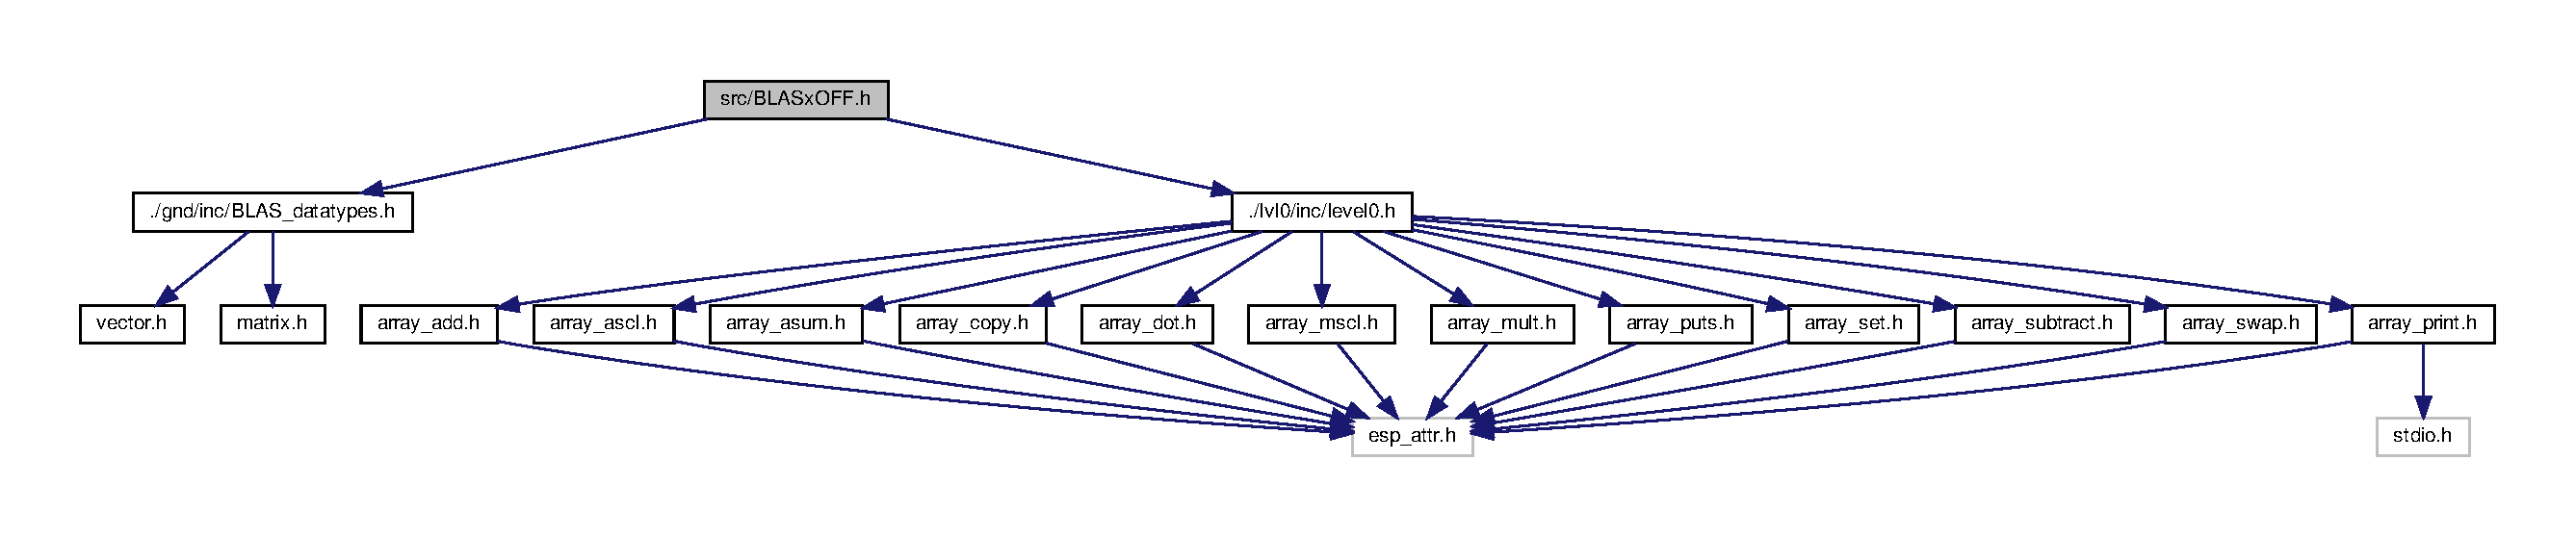
\includegraphics[width=350pt]{BLASxOFF_8h__incl}
\end{center}
\end{figure}

\hypertarget{copy__BLAS_8h}{}\section{src/copy\+\_\+\+B\+L\+AS.h File Reference}
\label{copy__BLAS_8h}\index{src/copy\+\_\+\+B\+L\+A\+S.\+h@{src/copy\+\_\+\+B\+L\+A\+S.\+h}}
{\ttfamily \#include \char`\"{}./gnd/inc/\+B\+L\+A\+S\+\_\+datatypes.\+h\char`\"{}}\newline
{\ttfamily \#include \char`\"{}./lvl0/inc/level0.\+h\char`\"{}}\newline
Include dependency graph for copy\+\_\+\+B\+L\+A\+S.\+h\+:
\nopagebreak
\begin{figure}[H]
\begin{center}
\leavevmode
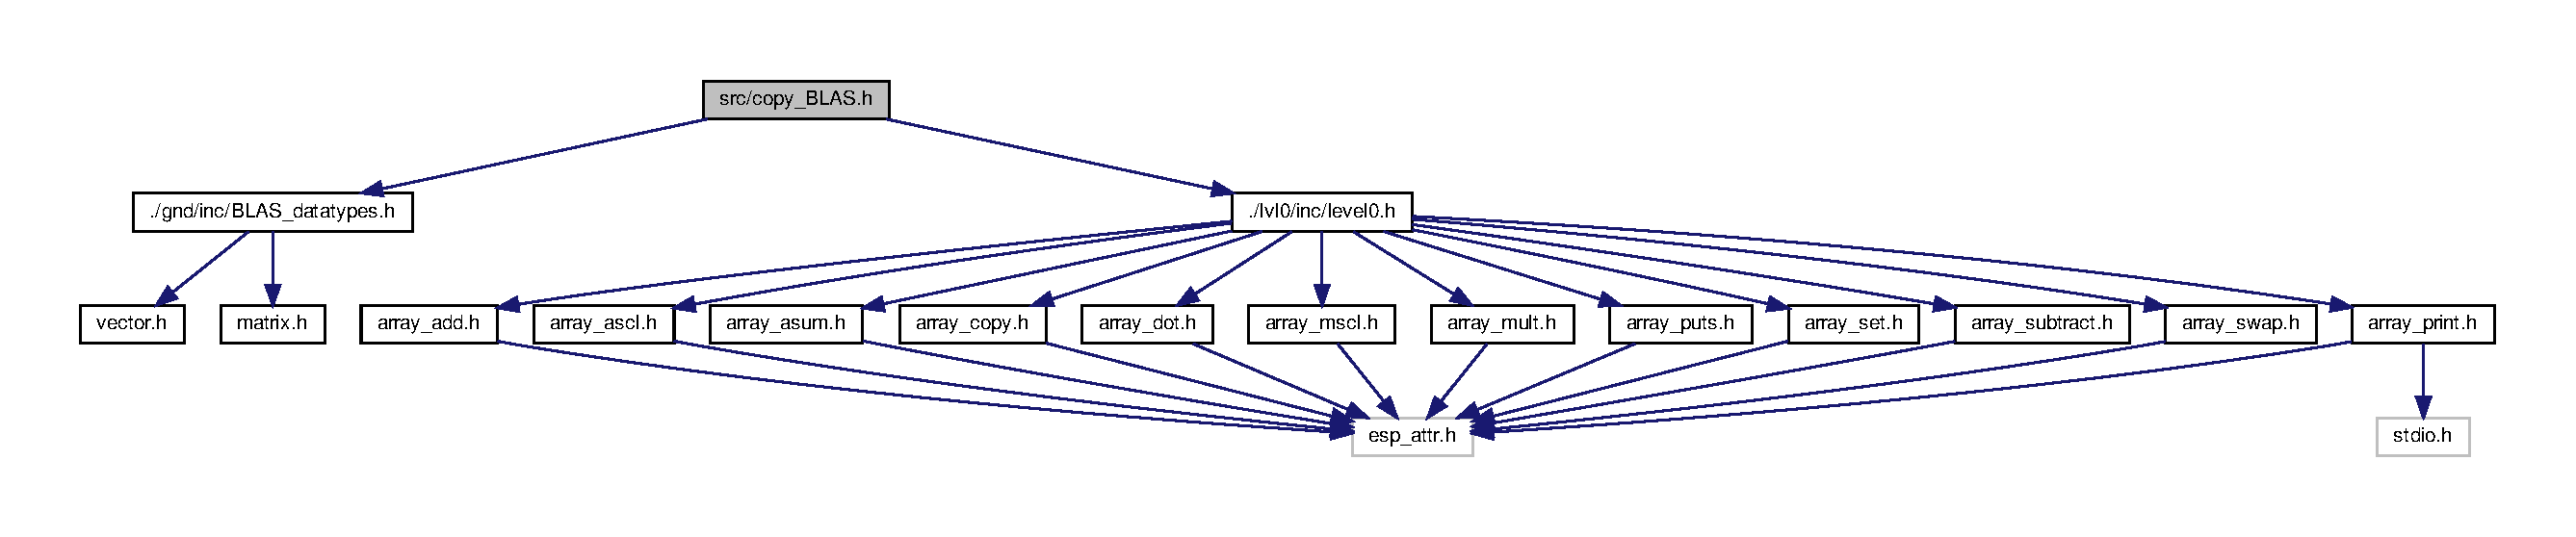
\includegraphics[width=350pt]{copy__BLAS_8h__incl}
\end{center}
\end{figure}

\hypertarget{BLAS__datatypes_8h}{}\section{src/gnd/inc/\+B\+L\+A\+S\+\_\+datatypes.h File Reference}
\label{BLAS__datatypes_8h}\index{src/gnd/inc/\+B\+L\+A\+S\+\_\+datatypes.\+h@{src/gnd/inc/\+B\+L\+A\+S\+\_\+datatypes.\+h}}
{\ttfamily \#include \char`\"{}vector.\+h\char`\"{}}\newline
{\ttfamily \#include \char`\"{}matrix.\+h\char`\"{}}\newline
Include dependency graph for B\+L\+A\+S\+\_\+datatypes.\+h\+:
\nopagebreak
\begin{figure}[H]
\begin{center}
\leavevmode
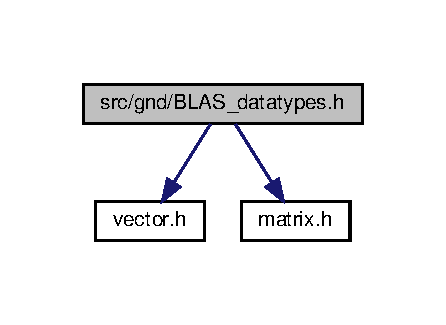
\includegraphics[width=229pt]{BLAS__datatypes_8h__incl}
\end{center}
\end{figure}
This graph shows which files directly or indirectly include this file\+:
\nopagebreak
\begin{figure}[H]
\begin{center}
\leavevmode
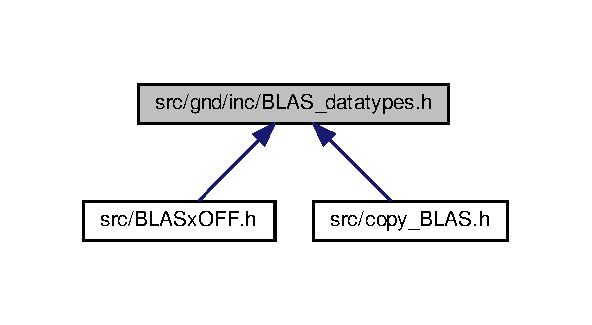
\includegraphics[width=284pt]{BLAS__datatypes_8h__dep__incl}
\end{center}
\end{figure}

\hypertarget{inc_2BLAS__datatypes_8h}{}\section{src/gnd/inc/\+B\+L\+A\+S\+\_\+datatypes.h File Reference}
\label{inc_2BLAS__datatypes_8h}\index{src/gnd/inc/\+B\+L\+A\+S\+\_\+datatypes.\+h@{src/gnd/inc/\+B\+L\+A\+S\+\_\+datatypes.\+h}}
{\ttfamily \#include \char`\"{}vector.\+h\char`\"{}}\newline
{\ttfamily \#include \char`\"{}matrix.\+h\char`\"{}}\newline
Include dependency graph for B\+L\+A\+S\+\_\+datatypes.\+h\+:\nopagebreak
\begin{figure}[H]
\begin{center}
\leavevmode
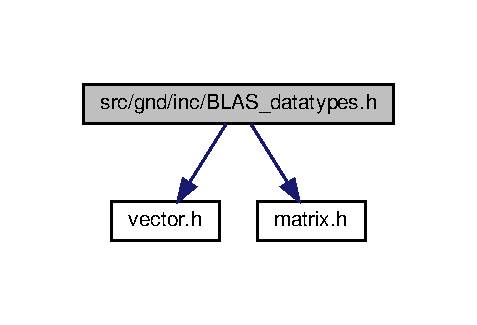
\includegraphics[width=229pt]{inc_2BLAS__datatypes_8h__incl}
\end{center}
\end{figure}
This graph shows which files directly or indirectly include this file\+:
\nopagebreak
\begin{figure}[H]
\begin{center}
\leavevmode
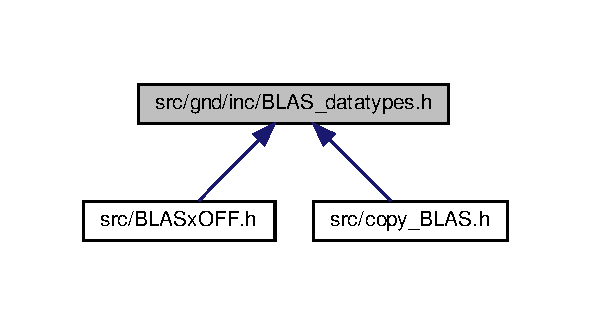
\includegraphics[width=284pt]{inc_2BLAS__datatypes_8h__dep__incl}
\end{center}
\end{figure}

\hypertarget{inc_2matrix_8h}{}\section{src/gnd/inc/matrix.h File Reference}
\label{inc_2matrix_8h}\index{src/gnd/inc/matrix.\+h@{src/gnd/inc/matrix.\+h}}
This graph shows which files directly or indirectly include this file\+:
\nopagebreak
\begin{figure}[H]
\begin{center}
\leavevmode
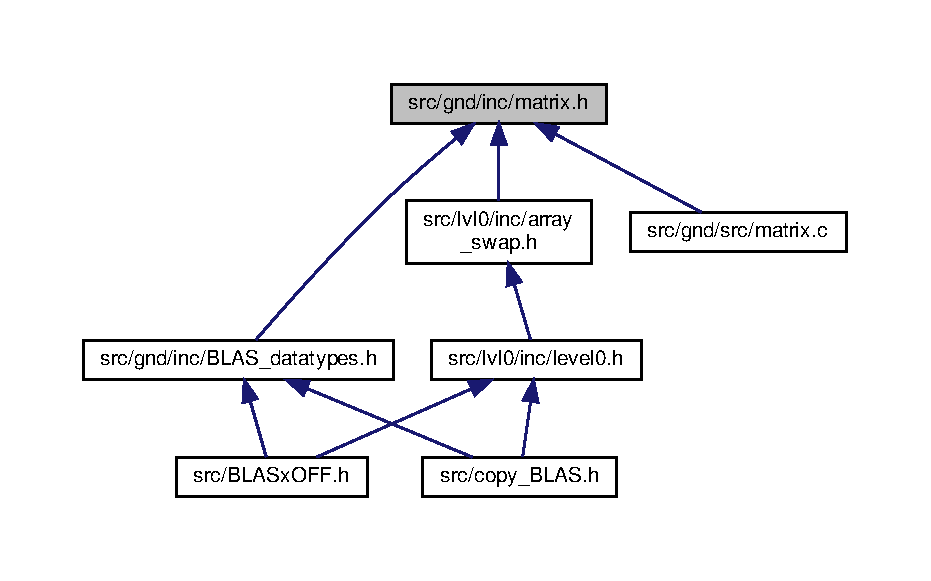
\includegraphics[width=350pt]{inc_2matrix_8h__dep__incl}
\end{center}
\end{figure}
\subsection*{Data Structures}
\begin{DoxyCompactItemize}
\item 
struct \hyperlink{structmatrix}{matrix}
\end{DoxyCompactItemize}
\subsection*{Macros}
\begin{DoxyCompactItemize}
\item 
\#define \hyperlink{inc_2matrix_8h_ac07aef2092efa03fbc087947d3abcba2}{M\+\_\+\+A\+L\+L\+O\+C\+A\+T\+E\+D\+\_\+F}~1
\begin{DoxyCompactList}\small\item\em Set flag for matrix allocation. \end{DoxyCompactList}\end{DoxyCompactItemize}
\subsection*{Variables}
\begin{DoxyCompactItemize}
\item 
struct \hyperlink{structmatrix}{matrix} \hyperlink{inc_2matrix_8h_a11394bf5c56be5e0348b6460f0d04aa0}{new\+\_\+matrix}
\end{DoxyCompactItemize}


\subsection{Macro Definition Documentation}
\mbox{\Hypertarget{inc_2matrix_8h_ac07aef2092efa03fbc087947d3abcba2}\label{inc_2matrix_8h_ac07aef2092efa03fbc087947d3abcba2}} 
\index{inc/matrix.\+h@{inc/matrix.\+h}!M\+\_\+\+A\+L\+L\+O\+C\+A\+T\+E\+D\+\_\+F@{M\+\_\+\+A\+L\+L\+O\+C\+A\+T\+E\+D\+\_\+F}}
\index{M\+\_\+\+A\+L\+L\+O\+C\+A\+T\+E\+D\+\_\+F@{M\+\_\+\+A\+L\+L\+O\+C\+A\+T\+E\+D\+\_\+F}!inc/matrix.\+h@{inc/matrix.\+h}}
\subsubsection{\texorpdfstring{M\+\_\+\+A\+L\+L\+O\+C\+A\+T\+E\+D\+\_\+F}{M\_ALLOCATED\_F}}
{\footnotesize\ttfamily \#define M\+\_\+\+A\+L\+L\+O\+C\+A\+T\+E\+D\+\_\+F~1}



Set flag for matrix allocation. 

Data type for Matricies used in Linear Algebra 

\subsection{Variable Documentation}
\mbox{\Hypertarget{inc_2matrix_8h_a11394bf5c56be5e0348b6460f0d04aa0}\label{inc_2matrix_8h_a11394bf5c56be5e0348b6460f0d04aa0}} 
\index{inc/matrix.\+h@{inc/matrix.\+h}!new\+\_\+matrix@{new\+\_\+matrix}}
\index{new\+\_\+matrix@{new\+\_\+matrix}!inc/matrix.\+h@{inc/matrix.\+h}}
\subsubsection{\texorpdfstring{new\+\_\+matrix}{new\_matrix}}
{\footnotesize\ttfamily struct \hyperlink{structmatrix}{matrix} new\+\_\+matrix}

Used to initilize matrix on call

Easy Zero-\/initializer for when making a new matrix 
\hypertarget{matrix_8h}{}\section{src/gnd/inc/matrix.h File Reference}
\label{matrix_8h}\index{src/gnd/inc/matrix.\+h@{src/gnd/inc/matrix.\+h}}
This graph shows which files directly or indirectly include this file\+:
\nopagebreak
\begin{figure}[H]
\begin{center}
\leavevmode
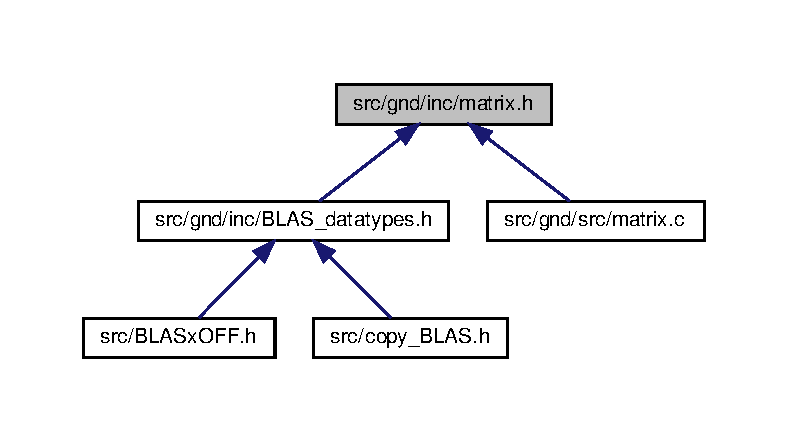
\includegraphics[width=350pt]{matrix_8h__dep__incl}
\end{center}
\end{figure}
\subsection*{Data Structures}
\begin{DoxyCompactItemize}
\item 
struct \hyperlink{structmatrix}{matrix}
\end{DoxyCompactItemize}
\subsection*{Macros}
\begin{DoxyCompactItemize}
\item 
\#define \hyperlink{matrix_8h_ac07aef2092efa03fbc087947d3abcba2}{M\+\_\+\+A\+L\+L\+O\+C\+A\+T\+E\+D\+\_\+F}~1
\begin{DoxyCompactList}\small\item\em Set flag for matrix allocation. \end{DoxyCompactList}\end{DoxyCompactItemize}
\subsection*{Variables}
\begin{DoxyCompactItemize}
\item 
struct \hyperlink{structmatrix}{matrix} \hyperlink{matrix_8h_a11394bf5c56be5e0348b6460f0d04aa0}{new\+\_\+matrix}
\end{DoxyCompactItemize}


\subsection{Macro Definition Documentation}
\mbox{\Hypertarget{matrix_8h_ac07aef2092efa03fbc087947d3abcba2}\label{matrix_8h_ac07aef2092efa03fbc087947d3abcba2}} 
\index{matrix.\+h@{matrix.\+h}!M\+\_\+\+A\+L\+L\+O\+C\+A\+T\+E\+D\+\_\+F@{M\+\_\+\+A\+L\+L\+O\+C\+A\+T\+E\+D\+\_\+F}}
\index{M\+\_\+\+A\+L\+L\+O\+C\+A\+T\+E\+D\+\_\+F@{M\+\_\+\+A\+L\+L\+O\+C\+A\+T\+E\+D\+\_\+F}!matrix.\+h@{matrix.\+h}}
\subsubsection{\texorpdfstring{M\+\_\+\+A\+L\+L\+O\+C\+A\+T\+E\+D\+\_\+F}{M\_ALLOCATED\_F}}
{\footnotesize\ttfamily \#define M\+\_\+\+A\+L\+L\+O\+C\+A\+T\+E\+D\+\_\+F~1}



Set flag for matrix allocation. 

Data type for Matricies used in Linear Algebra 

\subsection{Variable Documentation}
\mbox{\Hypertarget{matrix_8h_a11394bf5c56be5e0348b6460f0d04aa0}\label{matrix_8h_a11394bf5c56be5e0348b6460f0d04aa0}} 
\index{matrix.\+h@{matrix.\+h}!new\+\_\+matrix@{new\+\_\+matrix}}
\index{new\+\_\+matrix@{new\+\_\+matrix}!matrix.\+h@{matrix.\+h}}
\subsubsection{\texorpdfstring{new\+\_\+matrix}{new\_matrix}}
{\footnotesize\ttfamily struct \hyperlink{structmatrix}{matrix} new\+\_\+matrix}

Used to initilize matrix on call

Easy Zero-\/initializer for when making a new matrix 
\hypertarget{inc_2vector_8h}{}\section{src/gnd/inc/vector.h File Reference}
\label{inc_2vector_8h}\index{src/gnd/inc/vector.\+h@{src/gnd/inc/vector.\+h}}
This graph shows which files directly or indirectly include this file\+:
\nopagebreak
\begin{figure}[H]
\begin{center}
\leavevmode
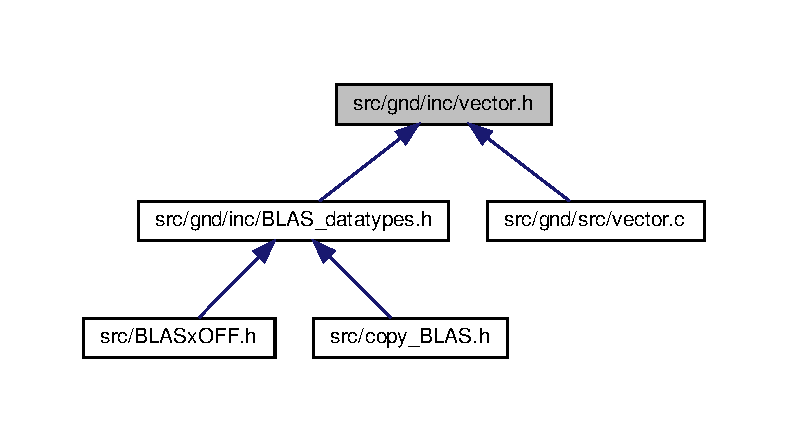
\includegraphics[width=350pt]{inc_2vector_8h__dep__incl}
\end{center}
\end{figure}
\subsection*{Data Structures}
\begin{DoxyCompactItemize}
\item 
struct \hyperlink{structvector}{vector}
\end{DoxyCompactItemize}
\subsection*{Macros}
\begin{DoxyCompactItemize}
\item 
\#define \hyperlink{inc_2vector_8h_a2566a6db3451171a78842272d28e9373}{V\+\_\+\+A\+L\+L\+O\+C\+A\+T\+E\+D\+\_\+F}~1
\begin{DoxyCompactList}\small\item\em Set flag for vector allocation. \end{DoxyCompactList}\end{DoxyCompactItemize}
\subsection*{Variables}
\begin{DoxyCompactItemize}
\item 
struct \hyperlink{structvector}{vector} \hyperlink{inc_2vector_8h_ae0d8044d4d9327f9ecae82ae077e57ea}{new\+\_\+vector}
\end{DoxyCompactItemize}


\subsection{Macro Definition Documentation}
\mbox{\Hypertarget{inc_2vector_8h_a2566a6db3451171a78842272d28e9373}\label{inc_2vector_8h_a2566a6db3451171a78842272d28e9373}} 
\index{inc/vector.\+h@{inc/vector.\+h}!V\+\_\+\+A\+L\+L\+O\+C\+A\+T\+E\+D\+\_\+F@{V\+\_\+\+A\+L\+L\+O\+C\+A\+T\+E\+D\+\_\+F}}
\index{V\+\_\+\+A\+L\+L\+O\+C\+A\+T\+E\+D\+\_\+F@{V\+\_\+\+A\+L\+L\+O\+C\+A\+T\+E\+D\+\_\+F}!inc/vector.\+h@{inc/vector.\+h}}
\subsubsection{\texorpdfstring{V\+\_\+\+A\+L\+L\+O\+C\+A\+T\+E\+D\+\_\+F}{V\_ALLOCATED\_F}}
{\footnotesize\ttfamily \#define V\+\_\+\+A\+L\+L\+O\+C\+A\+T\+E\+D\+\_\+F~1}



Set flag for vector allocation. 

Data type for Vatricies used in Linear Algebra 

\subsection{Variable Documentation}
\mbox{\Hypertarget{inc_2vector_8h_ae0d8044d4d9327f9ecae82ae077e57ea}\label{inc_2vector_8h_ae0d8044d4d9327f9ecae82ae077e57ea}} 
\index{inc/vector.\+h@{inc/vector.\+h}!new\+\_\+vector@{new\+\_\+vector}}
\index{new\+\_\+vector@{new\+\_\+vector}!inc/vector.\+h@{inc/vector.\+h}}
\subsubsection{\texorpdfstring{new\+\_\+vector}{new\_vector}}
{\footnotesize\ttfamily struct \hyperlink{structvector}{vector} new\+\_\+vector}

Used to initilize vector on call

Easy Zero-\/initializer for when making a new matrix 
\hypertarget{vector_8h}{}\section{src/gnd/vector.h File Reference}
\label{vector_8h}\index{src/gnd/vector.\+h@{src/gnd/vector.\+h}}
This graph shows which files directly or indirectly include this file\+:\nopagebreak
\begin{figure}[H]
\begin{center}
\leavevmode
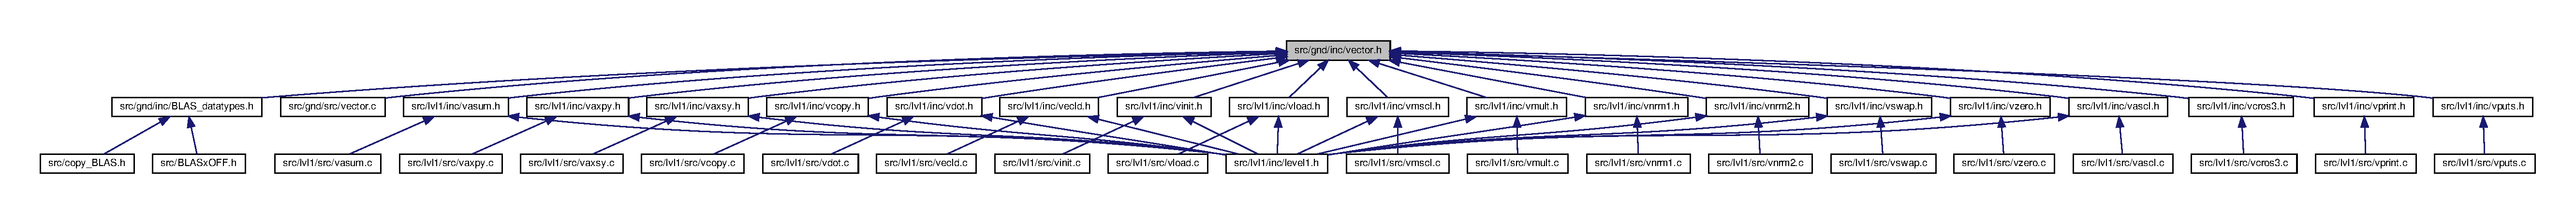
\includegraphics[width=214pt]{vector_8h__dep__incl}
\end{center}
\end{figure}
\subsection*{Data Structures}
\begin{DoxyCompactItemize}
\item 
struct \hyperlink{structvector}{vector}
\end{DoxyCompactItemize}
\subsection*{Macros}
\begin{DoxyCompactItemize}
\item 
\#define \hyperlink{vector_8h_a2566a6db3451171a78842272d28e9373}{V\+\_\+\+A\+L\+L\+O\+C\+A\+T\+E\+D\+\_\+F}~1
\begin{DoxyCompactList}\small\item\em Set flag for vector allocation. \end{DoxyCompactList}\end{DoxyCompactItemize}
\subsection*{Variables}
\begin{DoxyCompactItemize}
\item 
struct \hyperlink{structvector}{vector} \hyperlink{vector_8h_ae0d8044d4d9327f9ecae82ae077e57ea}{new\+\_\+vector}
\end{DoxyCompactItemize}


\subsection{Macro Definition Documentation}
\mbox{\Hypertarget{vector_8h_a2566a6db3451171a78842272d28e9373}\label{vector_8h_a2566a6db3451171a78842272d28e9373}} 
\index{vector.\+h@{vector.\+h}!V\+\_\+\+A\+L\+L\+O\+C\+A\+T\+E\+D\+\_\+F@{V\+\_\+\+A\+L\+L\+O\+C\+A\+T\+E\+D\+\_\+F}}
\index{V\+\_\+\+A\+L\+L\+O\+C\+A\+T\+E\+D\+\_\+F@{V\+\_\+\+A\+L\+L\+O\+C\+A\+T\+E\+D\+\_\+F}!vector.\+h@{vector.\+h}}
\subsubsection{\texorpdfstring{V\+\_\+\+A\+L\+L\+O\+C\+A\+T\+E\+D\+\_\+F}{V\_ALLOCATED\_F}}
{\footnotesize\ttfamily \#define V\+\_\+\+A\+L\+L\+O\+C\+A\+T\+E\+D\+\_\+F~1}



Set flag for vector allocation. 

Data type for Vatricies used in Linear Algebra 

\subsection{Variable Documentation}
\mbox{\Hypertarget{vector_8h_ae0d8044d4d9327f9ecae82ae077e57ea}\label{vector_8h_ae0d8044d4d9327f9ecae82ae077e57ea}} 
\index{vector.\+h@{vector.\+h}!new\+\_\+vector@{new\+\_\+vector}}
\index{new\+\_\+vector@{new\+\_\+vector}!vector.\+h@{vector.\+h}}
\subsubsection{\texorpdfstring{new\+\_\+vector}{new\_vector}}
{\footnotesize\ttfamily struct \hyperlink{structvector}{vector} new\+\_\+vector}

Used to initilize vector on call

Easy Zero-\/initializer for when making a new matrix 
\hypertarget{matrix_8c}{}\section{src/gnd/src/matrix.c File Reference}
\label{matrix_8c}\index{src/gnd/src/matrix.\+c@{src/gnd/src/matrix.\+c}}
{\ttfamily \#include $<$stddef.\+h$>$}\newline
{\ttfamily \#include \char`\"{}../inc/matrix.\+h\char`\"{}}\newline
Include dependency graph for matrix.\+c\+:\nopagebreak
\begin{figure}[H]
\begin{center}
\leavevmode
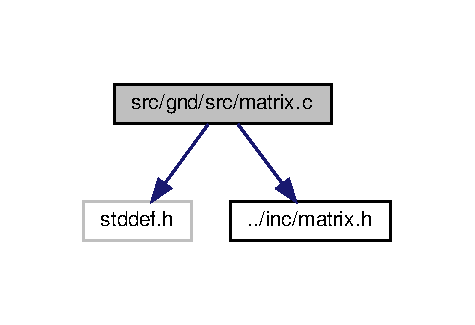
\includegraphics[width=228pt]{matrix_8c__incl}
\end{center}
\end{figure}
\subsection*{Variables}
\begin{DoxyCompactItemize}
\item 
struct \hyperlink{structmatrix}{matrix} \hyperlink{matrix_8c_a11394bf5c56be5e0348b6460f0d04aa0}{new\+\_\+matrix}
\end{DoxyCompactItemize}


\subsection{Variable Documentation}
\mbox{\Hypertarget{matrix_8c_a11394bf5c56be5e0348b6460f0d04aa0}\label{matrix_8c_a11394bf5c56be5e0348b6460f0d04aa0}} 
\index{matrix.\+c@{matrix.\+c}!new\+\_\+matrix@{new\+\_\+matrix}}
\index{new\+\_\+matrix@{new\+\_\+matrix}!matrix.\+c@{matrix.\+c}}
\subsubsection{\texorpdfstring{new\+\_\+matrix}{new\_matrix}}
{\footnotesize\ttfamily struct \hyperlink{structmatrix}{matrix} new\+\_\+matrix}

{\bfseries Initial value\+:}
\begin{DoxyCode}
= \{
  .flags = 0,
  .r = 0,
  .c = 0,
  .l = 0,
  .name = NULL,
  .m = NULL,
\}
\end{DoxyCode}
Easy Zero-\/initializer for when making a new matrix 
\hypertarget{vector_8c}{}\section{src/gnd/src/vector.c File Reference}
\label{vector_8c}\index{src/gnd/src/vector.\+c@{src/gnd/src/vector.\+c}}
{\ttfamily \#include $<$stddef.\+h$>$}\newline
{\ttfamily \#include \char`\"{}../inc/vector.\+h\char`\"{}}\newline
Include dependency graph for vector.\+c\+:\nopagebreak
\begin{figure}[H]
\begin{center}
\leavevmode
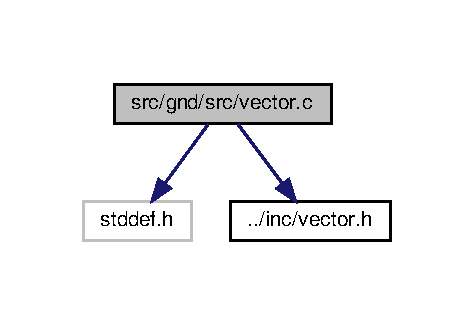
\includegraphics[width=228pt]{vector_8c__incl}
\end{center}
\end{figure}
\subsection*{Variables}
\begin{DoxyCompactItemize}
\item 
struct \hyperlink{structvector}{vector} \hyperlink{vector_8c_ae0d8044d4d9327f9ecae82ae077e57ea}{new\+\_\+vector}
\end{DoxyCompactItemize}


\subsection{Variable Documentation}
\mbox{\Hypertarget{vector_8c_ae0d8044d4d9327f9ecae82ae077e57ea}\label{vector_8c_ae0d8044d4d9327f9ecae82ae077e57ea}} 
\index{vector.\+c@{vector.\+c}!new\+\_\+vector@{new\+\_\+vector}}
\index{new\+\_\+vector@{new\+\_\+vector}!vector.\+c@{vector.\+c}}
\subsubsection{\texorpdfstring{new\+\_\+vector}{new\_vector}}
{\footnotesize\ttfamily struct \hyperlink{structvector}{vector} new\+\_\+vector}

{\bfseries Initial value\+:}
\begin{DoxyCode}
= \{
  .flags = 0,
  .l = 0,
  .v = NULL,
\}
\end{DoxyCode}
Easy Zero-\/initializer for when making a new matrix 
\hypertarget{array__add_8h}{}\section{src/lvl0/inc/array\+\_\+add.h File Reference}
\label{array__add_8h}\index{src/lvl0/inc/array\+\_\+add.\+h@{src/lvl0/inc/array\+\_\+add.\+h}}
{\ttfamily \#include \char`\"{}esp\+\_\+attr.\+h\char`\"{}}\newline
{\ttfamily \#include \char`\"{}../src/array\+\_\+add.\+c\char`\"{}}\newline
Include dependency graph for array\+\_\+add.\+h\+:\nopagebreak
\begin{figure}[H]
\begin{center}
\leavevmode
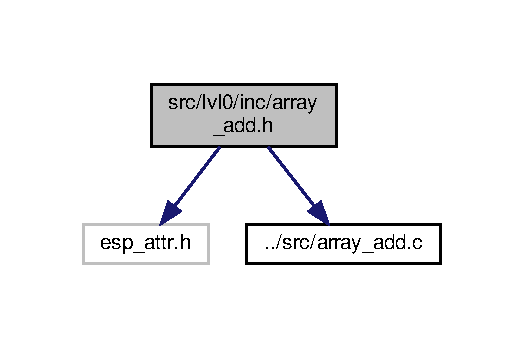
\includegraphics[width=252pt]{array__add_8h__incl}
\end{center}
\end{figure}
This graph shows which files directly or indirectly include this file\+:
\nopagebreak
\begin{figure}[H]
\begin{center}
\leavevmode
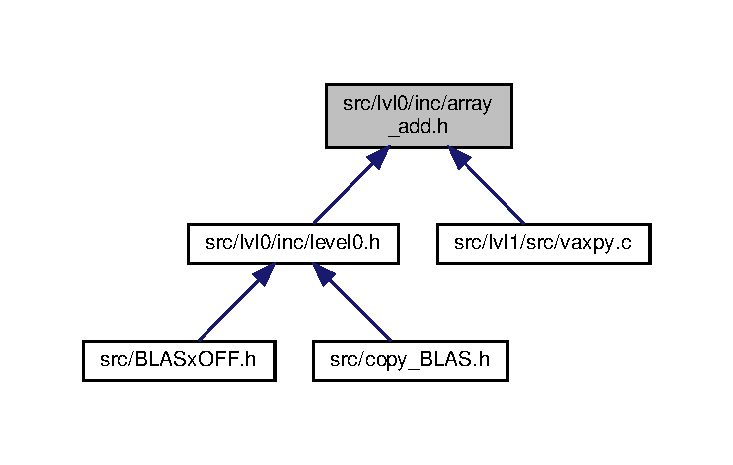
\includegraphics[width=284pt]{array__add_8h__dep__incl}
\end{center}
\end{figure}
\subsection*{Functions}
\begin{DoxyCompactItemize}
\item 
void I\+R\+A\+M\+\_\+\+A\+T\+TR \hyperlink{array__add_8h_a15b992b0dbde8612a35532df8efd7b4d}{array\+\_\+add} (float $\ast$arr\+Res, const float $\ast$arr\+OprA, const float $\ast$arr\+OprB, const unsigned int start, const unsigned int end) \+\_\+\+\_\+attribute\+\_\+\+\_\+((always\+\_\+inline)) \+\_\+\+\_\+attribute\+\_\+\+\_\+((nonull))
\end{DoxyCompactItemize}


\subsection{Function Documentation}
\mbox{\Hypertarget{array__add_8h_a15b992b0dbde8612a35532df8efd7b4d}\label{array__add_8h_a15b992b0dbde8612a35532df8efd7b4d}} 
\index{array\+\_\+add.\+h@{array\+\_\+add.\+h}!array\+\_\+add@{array\+\_\+add}}
\index{array\+\_\+add@{array\+\_\+add}!array\+\_\+add.\+h@{array\+\_\+add.\+h}}
\subsubsection{\texorpdfstring{array\+\_\+add()}{array\_add()}}
{\footnotesize\ttfamily void I\+R\+A\+M\+\_\+\+A\+T\+TR array\+\_\+add (\begin{DoxyParamCaption}\item[{float $\ast$}]{arr\+Res,  }\item[{const float $\ast$}]{arr\+OprA,  }\item[{const float $\ast$}]{arr\+OprB,  }\item[{const unsigned int}]{start,  }\item[{const unsigned int}]{end }\end{DoxyParamCaption})}

This function add two arrays together element by element 
\begin{DoxyParams}{Parameters}
{\em arr\+Res} & Array pointer where the result will be stored \\
\hline
{\em arr\+OprA} & Array pointer for the 1st operand \\
\hline
{\em arr\+OprB} & Array pointer for the 2nd operand \\
\hline
{\em start} & Starting element index to loop across \\
\hline
{\em end} & Last element index to loop across \\
\hline
\end{DoxyParams}

\hypertarget{array__ascl_8h}{}\section{src/lvl0/inc/array\+\_\+ascl.h File Reference}
\label{array__ascl_8h}\index{src/lvl0/inc/array\+\_\+ascl.\+h@{src/lvl0/inc/array\+\_\+ascl.\+h}}
{\ttfamily \#include \char`\"{}esp\+\_\+attr.\+h\char`\"{}}\newline
Include dependency graph for array\+\_\+ascl.\+h\+:
\nopagebreak
\begin{figure}[H]
\begin{center}
\leavevmode
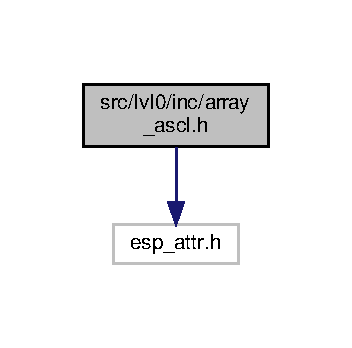
\includegraphics[width=169pt]{array__ascl_8h__incl}
\end{center}
\end{figure}
This graph shows which files directly or indirectly include this file\+:
\nopagebreak
\begin{figure}[H]
\begin{center}
\leavevmode
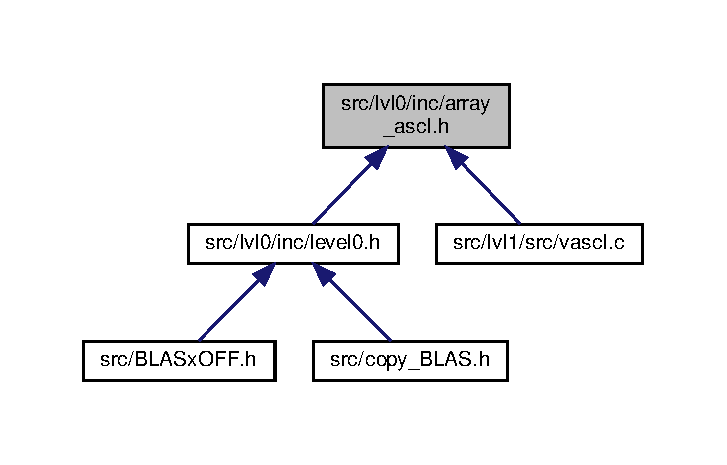
\includegraphics[width=349pt]{array__ascl_8h__dep__incl}
\end{center}
\end{figure}
\subsection*{Functions}
\begin{DoxyCompactItemize}
\item 
void I\+R\+A\+M\+\_\+\+A\+T\+TR \hyperlink{array__ascl_8h_a2cd5fcee5a0a6d5d582583da1daa095b}{\+\_\+\+\_\+attribute\+\_\+\+\_\+} ((always\+\_\+inline)) \+\_\+\+\_\+attribute\+\_\+\+\_\+((nonull)) array\+\_\+ascl(float $\ast$arr\+Res
\end{DoxyCompactItemize}
\subsection*{Variables}
\begin{DoxyCompactItemize}
\item 
void I\+R\+A\+M\+\_\+\+A\+T\+TR const float $\ast$ \hyperlink{array__ascl_8h_a951b57ce1d7dd691d9a66eda776f43f6}{arr\+Opr}
\begin{DoxyCompactList}\small\item\em $<$ Array pointer where the result will be stored \end{DoxyCompactList}\item 
void I\+R\+A\+M\+\_\+\+A\+T\+TR const float const float \hyperlink{array__ascl_8h_a8beac99f3a0446385106d145d3de1f90}{scl\+Opr}
\begin{DoxyCompactList}\small\item\em Scalar operand to add to the elements of the array operand. \end{DoxyCompactList}\item 
void I\+R\+A\+M\+\_\+\+A\+T\+TR const float const float const unsigned int \hyperlink{array__ascl_8h_a0549b2187026de7f72c6b3214fa437d5}{start}
\begin{DoxyCompactList}\small\item\em Begining element index to begin loop. \end{DoxyCompactList}\item 
void I\+R\+A\+M\+\_\+\+A\+T\+TR const float const float const unsigned int const unsigned int \hyperlink{array__ascl_8h_a68c28899964e31626b3c9e42853f0d42}{end}
\begin{DoxyCompactList}\small\item\em $<$ Last element index to loop across \end{DoxyCompactList}\end{DoxyCompactItemize}


\subsection{Function Documentation}
\mbox{\Hypertarget{array__ascl_8h_a2cd5fcee5a0a6d5d582583da1daa095b}\label{array__ascl_8h_a2cd5fcee5a0a6d5d582583da1daa095b}} 
\index{array\+\_\+ascl.\+h@{array\+\_\+ascl.\+h}!\+\_\+\+\_\+attribute\+\_\+\+\_\+@{\+\_\+\+\_\+attribute\+\_\+\+\_\+}}
\index{\+\_\+\+\_\+attribute\+\_\+\+\_\+@{\+\_\+\+\_\+attribute\+\_\+\+\_\+}!array\+\_\+ascl.\+h@{array\+\_\+ascl.\+h}}
\subsubsection{\texorpdfstring{\+\_\+\+\_\+attribute\+\_\+\+\_\+()}{\_\_attribute\_\_()}}
{\footnotesize\ttfamily void I\+R\+A\+M\+\_\+\+A\+T\+TR \+\_\+\+\_\+attribute\+\_\+\+\_\+ (\begin{DoxyParamCaption}\item[{(always\+\_\+inline)}]{ }\end{DoxyParamCaption})\hspace{0.3cm}{\ttfamily [inline]}}

This function adds a scalar too each element in an array


\begin{DoxyItemize}
\item This function is deliberatly placed in Instruction R\+AM. Meaning that this function will always remained cached.
\item the {\bfseries attribute}((always\+\_\+inline)) tells the compiler to A\+L\+W\+A\+YS inline to function reguardless of optimization levels
\item the {\bfseries attribute}((nonull)) tells the compiler that the function\textquotesingle{}s pointer arguments cannot bell N\+U\+LL 
\end{DoxyItemize}

\subsection{Variable Documentation}
\mbox{\Hypertarget{array__ascl_8h_a951b57ce1d7dd691d9a66eda776f43f6}\label{array__ascl_8h_a951b57ce1d7dd691d9a66eda776f43f6}} 
\index{array\+\_\+ascl.\+h@{array\+\_\+ascl.\+h}!arr\+Opr@{arr\+Opr}}
\index{arr\+Opr@{arr\+Opr}!array\+\_\+ascl.\+h@{array\+\_\+ascl.\+h}}
\subsubsection{\texorpdfstring{arr\+Opr}{arrOpr}}
{\footnotesize\ttfamily void I\+R\+A\+M\+\_\+\+A\+T\+TR const float$\ast$ arr\+Opr}



$<$ Array pointer where the result will be stored 

Pointer for the array operand \mbox{\Hypertarget{array__ascl_8h_a68c28899964e31626b3c9e42853f0d42}\label{array__ascl_8h_a68c28899964e31626b3c9e42853f0d42}} 
\index{array\+\_\+ascl.\+h@{array\+\_\+ascl.\+h}!end@{end}}
\index{end@{end}!array\+\_\+ascl.\+h@{array\+\_\+ascl.\+h}}
\subsubsection{\texorpdfstring{end}{end}}
{\footnotesize\ttfamily void I\+R\+A\+M\+\_\+\+A\+T\+TR const float const float const unsigned int const unsigned int end}

{\bfseries Initial value\+:}
\begin{DoxyCode}
\{
    \textcolor{keywordflow}{for}(\textcolor{keywordtype}{unsigned} \textcolor{keywordtype}{int} I=\hyperlink{array__ascl_8h_a0549b2187026de7f72c6b3214fa437d5}{start}; I<\hyperlink{array__ascl_8h_a68c28899964e31626b3c9e42853f0d42}{end};++I) \{
      arrRes[I] = \hyperlink{array__ascl_8h_a951b57ce1d7dd691d9a66eda776f43f6}{arrOpr}[I] + \hyperlink{array__ascl_8h_a8beac99f3a0446385106d145d3de1f90}{sclOpr};
    \}
    \textcolor{keywordflow}{return}
\end{DoxyCode}


$<$ Last element index to loop across 

\mbox{\Hypertarget{array__ascl_8h_a8beac99f3a0446385106d145d3de1f90}\label{array__ascl_8h_a8beac99f3a0446385106d145d3de1f90}} 
\index{array\+\_\+ascl.\+h@{array\+\_\+ascl.\+h}!scl\+Opr@{scl\+Opr}}
\index{scl\+Opr@{scl\+Opr}!array\+\_\+ascl.\+h@{array\+\_\+ascl.\+h}}
\subsubsection{\texorpdfstring{scl\+Opr}{sclOpr}}
{\footnotesize\ttfamily void I\+R\+A\+M\+\_\+\+A\+T\+TR const float const float scl\+Opr}



Scalar operand to add to the elements of the array operand. 

\mbox{\Hypertarget{array__ascl_8h_a0549b2187026de7f72c6b3214fa437d5}\label{array__ascl_8h_a0549b2187026de7f72c6b3214fa437d5}} 
\index{array\+\_\+ascl.\+h@{array\+\_\+ascl.\+h}!start@{start}}
\index{start@{start}!array\+\_\+ascl.\+h@{array\+\_\+ascl.\+h}}
\subsubsection{\texorpdfstring{start}{start}}
{\footnotesize\ttfamily void I\+R\+A\+M\+\_\+\+A\+T\+TR const float const float const unsigned int start}



Begining element index to begin loop. 


\hypertarget{array__asum_8h}{}\section{src/lvl0/inc/array\+\_\+asum.h File Reference}
\label{array__asum_8h}\index{src/lvl0/inc/array\+\_\+asum.\+h@{src/lvl0/inc/array\+\_\+asum.\+h}}
{\ttfamily \#include \char`\"{}esp\+\_\+attr.\+h\char`\"{}}\newline
Include dependency graph for array\+\_\+asum.\+h\+:
\nopagebreak
\begin{figure}[H]
\begin{center}
\leavevmode
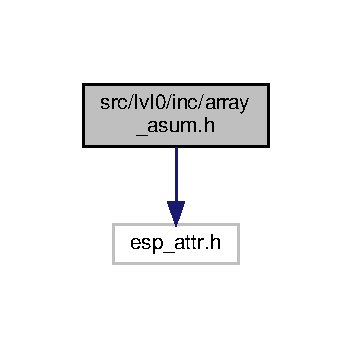
\includegraphics[width=169pt]{array__asum_8h__incl}
\end{center}
\end{figure}
This graph shows which files directly or indirectly include this file\+:
\nopagebreak
\begin{figure}[H]
\begin{center}
\leavevmode
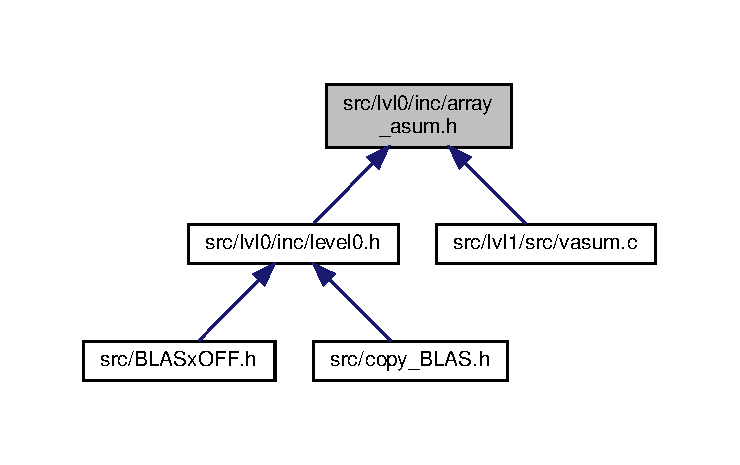
\includegraphics[width=350pt]{array__asum_8h__dep__incl}
\end{center}
\end{figure}
\subsection*{Functions}
\begin{DoxyCompactItemize}
\item 
void I\+R\+A\+M\+\_\+\+A\+T\+TR \hyperlink{array__asum_8h_af8fe767b6255bf4e9260b478c555a44f}{\+\_\+\+\_\+attribute\+\_\+\+\_\+} ((always\+\_\+inline)) \+\_\+\+\_\+attribute\+\_\+\+\_\+((nonull)) array\+\_\+asum(float $\ast$\hyperlink{array__dot_8h_a679c62e32495a27559a1723609a78a20}{scl\+Res}
\item 
\hyperlink{array__asum_8h_abe37ef39291fe27f977e30e3118c90f9}{for} (unsigned int I=\hyperlink{array__zero_8h_a1951879481f1ba4287d30b0a485429fc}{start};I$<$ \hyperlink{array__zero_8h_ae062d39ef5523e038e43c08fa9fe07b4}{end};++I)
\end{DoxyCompactItemize}
\subsection*{Variables}
\begin{DoxyCompactItemize}
\item 
void I\+R\+A\+M\+\_\+\+A\+T\+TR const float $\ast$ \hyperlink{array__asum_8h_a951b57ce1d7dd691d9a66eda776f43f6}{arr\+Opr}
\begin{DoxyCompactList}\small\item\em $<$ Float pointer for return value \end{DoxyCompactList}\item 
void I\+R\+A\+M\+\_\+\+A\+T\+TR const float const unsigned int \hyperlink{array__asum_8h_afd423ccb9a3b73eaf00854e74324938e}{start}
\begin{DoxyCompactList}\small\item\em Starting element index to loop across. \end{DoxyCompactList}\item 
void I\+R\+A\+M\+\_\+\+A\+T\+TR const float const unsigned int const unsigned int \hyperlink{array__asum_8h_a3827eeafb6094da9458f36d58f5e1f8e}{end}
\begin{DoxyCompactList}\small\item\em $<$ Last element index to loop across \end{DoxyCompactList}\item 
$\ast$ \hyperlink{array__asum_8h_a679c62e32495a27559a1723609a78a20}{scl\+Res} = res
\item 
\hyperlink{array__asum_8h_a9717e7bbecb906637e86cef6da3d83c2}{return}
\end{DoxyCompactItemize}


\subsection{Function Documentation}
\mbox{\Hypertarget{array__asum_8h_af8fe767b6255bf4e9260b478c555a44f}\label{array__asum_8h_af8fe767b6255bf4e9260b478c555a44f}} 
\index{array\+\_\+asum.\+h@{array\+\_\+asum.\+h}!\+\_\+\+\_\+attribute\+\_\+\+\_\+@{\+\_\+\+\_\+attribute\+\_\+\+\_\+}}
\index{\+\_\+\+\_\+attribute\+\_\+\+\_\+@{\+\_\+\+\_\+attribute\+\_\+\+\_\+}!array\+\_\+asum.\+h@{array\+\_\+asum.\+h}}
\subsubsection{\texorpdfstring{\+\_\+\+\_\+attribute\+\_\+\+\_\+()}{\_\_attribute\_\_()}}
{\footnotesize\ttfamily void I\+R\+A\+M\+\_\+\+A\+T\+TR \+\_\+\+\_\+attribute\+\_\+\+\_\+ (\begin{DoxyParamCaption}\item[{(always\+\_\+inline)}]{ }\end{DoxyParamCaption})\hspace{0.3cm}{\ttfamily [inline]}}

This function adds all the elements in an array and returns the sum \mbox{\Hypertarget{array__asum_8h_abe37ef39291fe27f977e30e3118c90f9}\label{array__asum_8h_abe37ef39291fe27f977e30e3118c90f9}} 
\index{array\+\_\+asum.\+h@{array\+\_\+asum.\+h}!for@{for}}
\index{for@{for}!array\+\_\+asum.\+h@{array\+\_\+asum.\+h}}
\subsubsection{\texorpdfstring{for()}{for()}}
{\footnotesize\ttfamily for (\begin{DoxyParamCaption}{ }\end{DoxyParamCaption})}



\subsection{Variable Documentation}
\mbox{\Hypertarget{array__asum_8h_a951b57ce1d7dd691d9a66eda776f43f6}\label{array__asum_8h_a951b57ce1d7dd691d9a66eda776f43f6}} 
\index{array\+\_\+asum.\+h@{array\+\_\+asum.\+h}!arr\+Opr@{arr\+Opr}}
\index{arr\+Opr@{arr\+Opr}!array\+\_\+asum.\+h@{array\+\_\+asum.\+h}}
\subsubsection{\texorpdfstring{arr\+Opr}{arrOpr}}
{\footnotesize\ttfamily void I\+R\+A\+M\+\_\+\+A\+T\+TR const float$\ast$ arr\+Opr}



$<$ Float pointer for return value 

Array pointer for elements to sum \mbox{\Hypertarget{array__asum_8h_a3827eeafb6094da9458f36d58f5e1f8e}\label{array__asum_8h_a3827eeafb6094da9458f36d58f5e1f8e}} 
\index{array\+\_\+asum.\+h@{array\+\_\+asum.\+h}!end@{end}}
\index{end@{end}!array\+\_\+asum.\+h@{array\+\_\+asum.\+h}}
\subsubsection{\texorpdfstring{end}{end}}
{\footnotesize\ttfamily void I\+R\+A\+M\+\_\+\+A\+T\+TR const float const unsigned int const unsigned int end}

{\bfseries Initial value\+:}
\begin{DoxyCode}
\{
    \textcolor{keywordtype}{float} res = 0.0
\end{DoxyCode}


$<$ Last element index to loop across 

\mbox{\Hypertarget{array__asum_8h_a9717e7bbecb906637e86cef6da3d83c2}\label{array__asum_8h_a9717e7bbecb906637e86cef6da3d83c2}} 
\index{array\+\_\+asum.\+h@{array\+\_\+asum.\+h}!return@{return}}
\index{return@{return}!array\+\_\+asum.\+h@{array\+\_\+asum.\+h}}
\subsubsection{\texorpdfstring{return}{return}}
{\footnotesize\ttfamily return}

\mbox{\Hypertarget{array__asum_8h_a679c62e32495a27559a1723609a78a20}\label{array__asum_8h_a679c62e32495a27559a1723609a78a20}} 
\index{array\+\_\+asum.\+h@{array\+\_\+asum.\+h}!scl\+Res@{scl\+Res}}
\index{scl\+Res@{scl\+Res}!array\+\_\+asum.\+h@{array\+\_\+asum.\+h}}
\subsubsection{\texorpdfstring{scl\+Res}{sclRes}}
{\footnotesize\ttfamily $\ast$ scl\+Res = res}

\mbox{\Hypertarget{array__asum_8h_afd423ccb9a3b73eaf00854e74324938e}\label{array__asum_8h_afd423ccb9a3b73eaf00854e74324938e}} 
\index{array\+\_\+asum.\+h@{array\+\_\+asum.\+h}!start@{start}}
\index{start@{start}!array\+\_\+asum.\+h@{array\+\_\+asum.\+h}}
\subsubsection{\texorpdfstring{start}{start}}
{\footnotesize\ttfamily void I\+R\+A\+M\+\_\+\+A\+T\+TR const float const unsigned int start}



Starting element index to loop across. 


\hypertarget{array__copy_8h}{}\section{src/lvl0/inc/array\+\_\+copy.h File Reference}
\label{array__copy_8h}\index{src/lvl0/inc/array\+\_\+copy.\+h@{src/lvl0/inc/array\+\_\+copy.\+h}}
{\ttfamily \#include \char`\"{}esp\+\_\+attr.\+h\char`\"{}}\newline
{\ttfamily \#include \char`\"{}../src/array\+\_\+copy.\+c\char`\"{}}\newline
Include dependency graph for array\+\_\+copy.\+h\+:\nopagebreak
\begin{figure}[H]
\begin{center}
\leavevmode
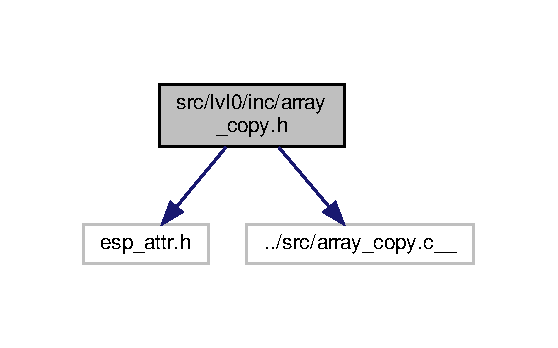
\includegraphics[width=256pt]{array__copy_8h__incl}
\end{center}
\end{figure}
This graph shows which files directly or indirectly include this file\+:
\nopagebreak
\begin{figure}[H]
\begin{center}
\leavevmode
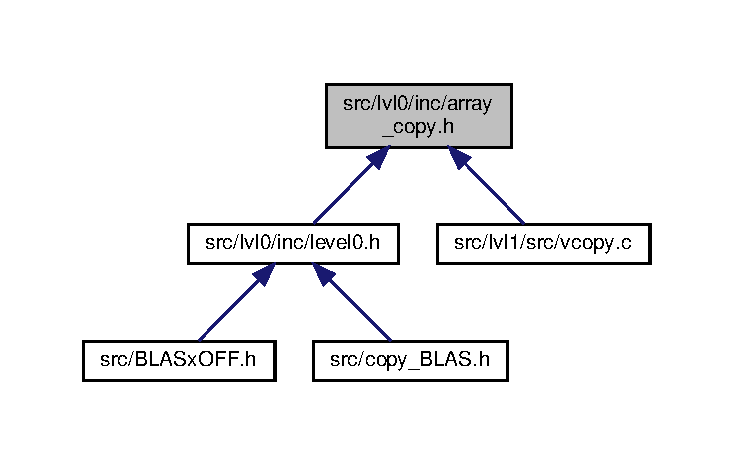
\includegraphics[width=350pt]{array__copy_8h__dep__incl}
\end{center}
\end{figure}
\subsection*{Functions}
\begin{DoxyCompactItemize}
\item 
void I\+R\+A\+M\+\_\+\+A\+T\+TR \hyperlink{array__copy_8h_a6eff457f740569ba50b92c95bd5193b1}{array\+\_\+copy} (float $\ast$arr\+Dst, const float $\ast$arr\+Src, const unsigned int start, const unsigned int end) \+\_\+\+\_\+attribute\+\_\+\+\_\+((always\+\_\+inline)) \+\_\+\+\_\+attribute\+\_\+\+\_\+((nonull))
\end{DoxyCompactItemize}


\subsection{Function Documentation}
\mbox{\Hypertarget{array__copy_8h_a6eff457f740569ba50b92c95bd5193b1}\label{array__copy_8h_a6eff457f740569ba50b92c95bd5193b1}} 
\index{array\+\_\+copy.\+h@{array\+\_\+copy.\+h}!array\+\_\+copy@{array\+\_\+copy}}
\index{array\+\_\+copy@{array\+\_\+copy}!array\+\_\+copy.\+h@{array\+\_\+copy.\+h}}
\subsubsection{\texorpdfstring{array\+\_\+copy()}{array\_copy()}}
{\footnotesize\ttfamily void I\+R\+A\+M\+\_\+\+A\+T\+TR array\+\_\+copy (\begin{DoxyParamCaption}\item[{float $\ast$}]{arr\+Dst,  }\item[{const float $\ast$}]{arr\+Src,  }\item[{const unsigned int}]{start,  }\item[{const unsigned int}]{end }\end{DoxyParamCaption})}

This function copies the elements of one arrays into another array 
\begin{DoxyParams}{Parameters}
{\em arr\+Dst} & Array pointer destination to copy source data into \\
\hline
{\em arr\+Src} & Array pointer for source data \\
\hline
{\em start} & Starting element index to loop across \\
\hline
{\em end} & Last element index to loop across \\
\hline
\end{DoxyParams}
Here is the caller graph for this function\+:
\nopagebreak
\begin{figure}[H]
\begin{center}
\leavevmode
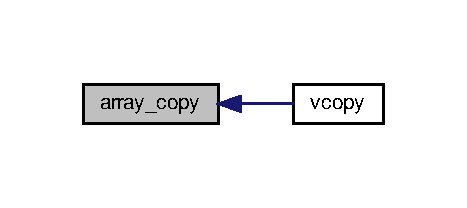
\includegraphics[width=224pt]{array__copy_8h_a6eff457f740569ba50b92c95bd5193b1_icgraph}
\end{center}
\end{figure}

\hypertarget{array__dot_8h}{}\section{src/lvl0/inc/array\+\_\+dot.h File Reference}
\label{array__dot_8h}\index{src/lvl0/inc/array\+\_\+dot.\+h@{src/lvl0/inc/array\+\_\+dot.\+h}}
{\ttfamily \#include \char`\"{}esp\+\_\+attr.\+h\char`\"{}}\newline
{\ttfamily \#include \char`\"{}../src/array\+\_\+dot.\+c\+\_\+\+\_\+\char`\"{}}\newline
Include dependency graph for array\+\_\+dot.\+h\+:
\nopagebreak
\begin{figure}[H]
\begin{center}
\leavevmode
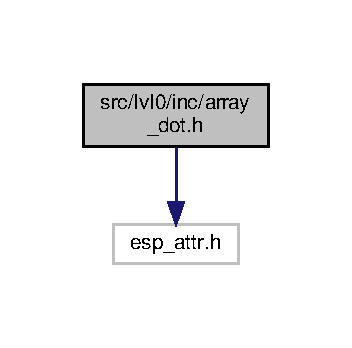
\includegraphics[width=260pt]{array__dot_8h__incl}
\end{center}
\end{figure}
This graph shows which files directly or indirectly include this file\+:
\nopagebreak
\begin{figure}[H]
\begin{center}
\leavevmode
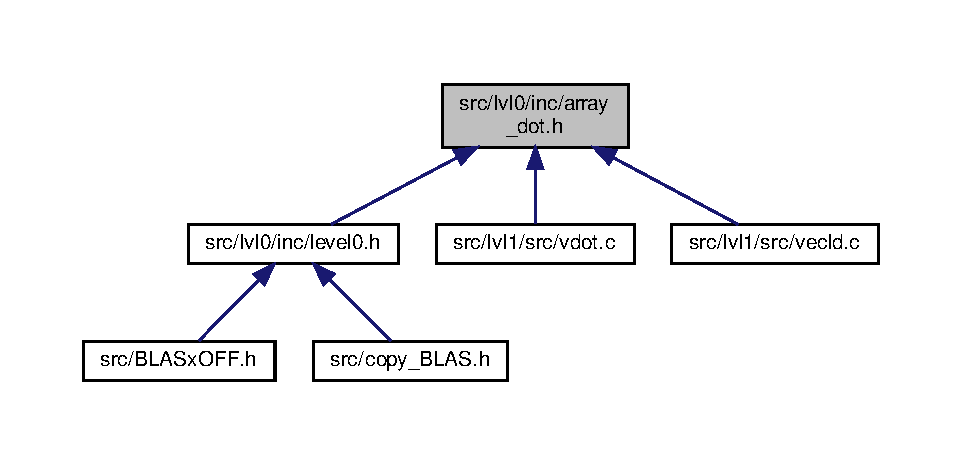
\includegraphics[width=345pt]{array__dot_8h__dep__incl}
\end{center}
\end{figure}
\subsection*{Functions}
\begin{DoxyCompactItemize}
\item 
void I\+R\+A\+M\+\_\+\+A\+T\+TR \hyperlink{array__dot_8h_a5f226f010b6fa6dc2111595f46e623b0}{array\+\_\+dot} (float $\ast$scl\+Res, const float $\ast$arr\+OprA, const float $\ast$arr\+OprB, const unsigned int start, const unsigned int end) \+\_\+\+\_\+attribute\+\_\+\+\_\+((always\+\_\+inline)) \+\_\+\+\_\+attribute\+\_\+\+\_\+((nonull))
\end{DoxyCompactItemize}


\subsection{Function Documentation}
\mbox{\Hypertarget{array__dot_8h_a5f226f010b6fa6dc2111595f46e623b0}\label{array__dot_8h_a5f226f010b6fa6dc2111595f46e623b0}} 
\index{array\+\_\+dot.\+h@{array\+\_\+dot.\+h}!array\+\_\+dot@{array\+\_\+dot}}
\index{array\+\_\+dot@{array\+\_\+dot}!array\+\_\+dot.\+h@{array\+\_\+dot.\+h}}
\subsubsection{\texorpdfstring{array\+\_\+dot()}{array\_dot()}}
{\footnotesize\ttfamily void I\+R\+A\+M\+\_\+\+A\+T\+TR array\+\_\+dot (\begin{DoxyParamCaption}\item[{float $\ast$}]{scl\+Res,  }\item[{const float $\ast$}]{arr\+OprA,  }\item[{const float $\ast$}]{arr\+OprB,  }\item[{const unsigned int}]{start,  }\item[{const unsigned int}]{end }\end{DoxyParamCaption})}

This function computes the dot product between two arrays 
\begin{DoxyParams}{Parameters}
{\em scl\+Res} & Array pointer where the result will be stored \\
\hline
{\em arr\+OprA} & Array pointer for the 1st operand \\
\hline
{\em arr\+OprB} & Array pointer for the 2nd operand \\
\hline
{\em start} & Starting element index to loop across \\
\hline
{\em end} & Last element index to loop across \\
\hline
\end{DoxyParams}
Here is the caller graph for this function\+:
\nopagebreak
\begin{figure}[H]
\begin{center}
\leavevmode
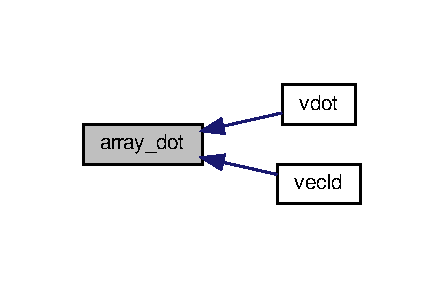
\includegraphics[width=208pt]{array__dot_8h_a5f226f010b6fa6dc2111595f46e623b0_icgraph}
\end{center}
\end{figure}

\hypertarget{array__mscl_8h}{}\section{src/lvl0/inc/array\+\_\+mscl.h File Reference}
\label{array__mscl_8h}\index{src/lvl0/inc/array\+\_\+mscl.\+h@{src/lvl0/inc/array\+\_\+mscl.\+h}}
{\ttfamily \#include \char`\"{}esp\+\_\+attr.\+h\char`\"{}}\newline
{\ttfamily \#include \char`\"{}../src/array\+\_\+mscl.\+c\char`\"{}}\newline
Include dependency graph for array\+\_\+mscl.\+h\+:\nopagebreak
\begin{figure}[H]
\begin{center}
\leavevmode
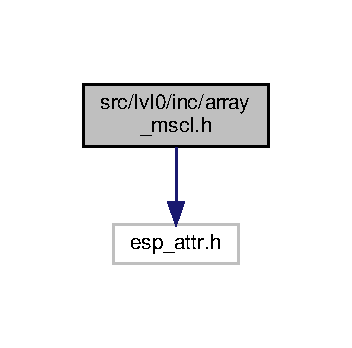
\includegraphics[width=256pt]{array__mscl_8h__incl}
\end{center}
\end{figure}
This graph shows which files directly or indirectly include this file\+:
\nopagebreak
\begin{figure}[H]
\begin{center}
\leavevmode
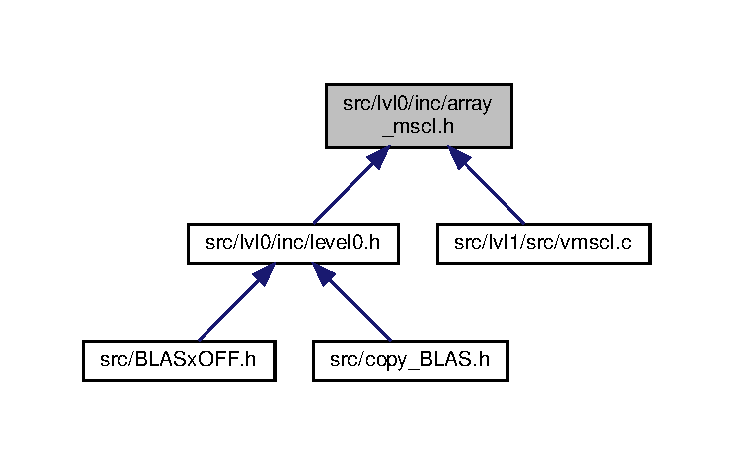
\includegraphics[width=284pt]{array__mscl_8h__dep__incl}
\end{center}
\end{figure}
\subsection*{Functions}
\begin{DoxyCompactItemize}
\item 
void I\+R\+A\+M\+\_\+\+A\+T\+TR \hyperlink{array__mscl_8h_a2fb8bc49731c026d4d80393cb780b8cf}{array\+\_\+mscl} (float $\ast$arr\+Res, const float $\ast$arr\+Opr, const unsigned int start, const unsigned int end, const float scl\+Opr) \+\_\+\+\_\+attribute\+\_\+\+\_\+((always\+\_\+inline)) \+\_\+\+\_\+attribute\+\_\+\+\_\+((nonull))
\end{DoxyCompactItemize}


\subsection{Function Documentation}
\mbox{\Hypertarget{array__mscl_8h_a2fb8bc49731c026d4d80393cb780b8cf}\label{array__mscl_8h_a2fb8bc49731c026d4d80393cb780b8cf}} 
\index{array\+\_\+mscl.\+h@{array\+\_\+mscl.\+h}!array\+\_\+mscl@{array\+\_\+mscl}}
\index{array\+\_\+mscl@{array\+\_\+mscl}!array\+\_\+mscl.\+h@{array\+\_\+mscl.\+h}}
\subsubsection{\texorpdfstring{array\+\_\+mscl()}{array\_mscl()}}
{\footnotesize\ttfamily void I\+R\+A\+M\+\_\+\+A\+T\+TR array\+\_\+mscl (\begin{DoxyParamCaption}\item[{float $\ast$}]{arr\+Res,  }\item[{const float $\ast$}]{arr\+Opr,  }\item[{const unsigned int}]{start,  }\item[{const unsigned int}]{end,  }\item[{const float}]{scl\+Opr }\end{DoxyParamCaption})}

This function multiplies each element of an array by a scalar 
\begin{DoxyParams}{Parameters}
{\em arr\+Res} & Array pointer where the result will be stored \\
\hline
{\em arr\+Opr} & Array pointer for the 1st operand \\
\hline
{\em start} & Starting element index to loop across \\
\hline
{\em end} & Last element index to loop across \\
\hline
{\em scl\+Opr} & float for the 2nd Scalar operand \\
\hline
\end{DoxyParams}

\hypertarget{array__mult_8h}{}\section{src/lvl0/inc/array\+\_\+mult.h File Reference}
\label{array__mult_8h}\index{src/lvl0/inc/array\+\_\+mult.\+h@{src/lvl0/inc/array\+\_\+mult.\+h}}
{\ttfamily \#include \char`\"{}esp\+\_\+attr.\+h\char`\"{}}\newline
Include dependency graph for array\+\_\+mult.\+h\+:
\nopagebreak
\begin{figure}[H]
\begin{center}
\leavevmode
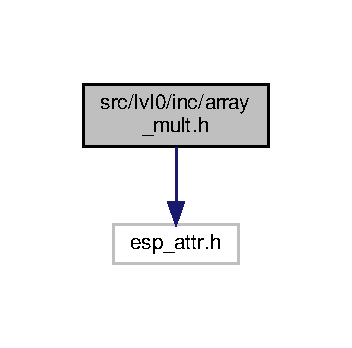
\includegraphics[width=169pt]{array__mult_8h__incl}
\end{center}
\end{figure}
This graph shows which files directly or indirectly include this file\+:
\nopagebreak
\begin{figure}[H]
\begin{center}
\leavevmode
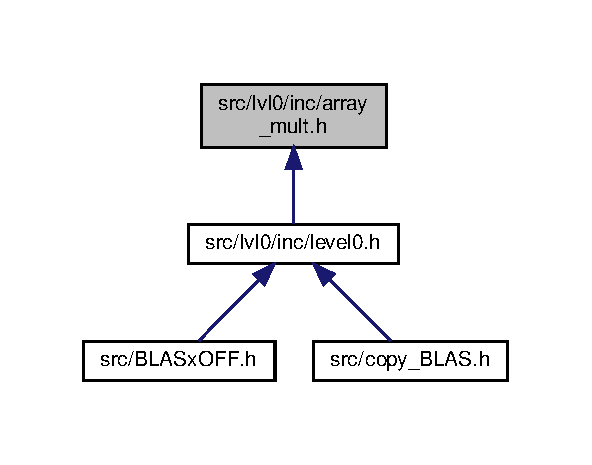
\includegraphics[width=350pt]{array__mult_8h__dep__incl}
\end{center}
\end{figure}
\subsection*{Macros}
\begin{DoxyCompactItemize}
\item 
\#define \hyperlink{array__mult_8h_ae6ff41290217771563cb86884152a2d0}{A\+R\+R\+A\+Y\+\_\+\+M\+U\+L\+T\+\_\+H}
\end{DoxyCompactItemize}
\subsection*{Functions}
\begin{DoxyCompactItemize}
\item 
void I\+R\+A\+M\+\_\+\+A\+T\+TR \hyperlink{array__mult_8h_a734470c4a3d399eca901aa8851286dbc}{\+\_\+\+\_\+attribute\+\_\+\+\_\+} ((always\+\_\+inline)) \+\_\+\+\_\+attribute\+\_\+\+\_\+((nonull)) array\+\_\+mult(float $\ast$arr\+Res
\end{DoxyCompactItemize}
\subsection*{Variables}
\begin{DoxyCompactItemize}
\item 
void I\+R\+A\+M\+\_\+\+A\+T\+TR const float $\ast$ \hyperlink{array__mult_8h_a5e4e071457fdcdd98fd22e75c6bfc555}{arr\+OprA}
\begin{DoxyCompactList}\small\item\em $<$ Array pointer where the result will be stored \end{DoxyCompactList}\item 
void I\+R\+A\+M\+\_\+\+A\+T\+TR const float const float $\ast$ \hyperlink{array__mult_8h_ad0fdcae3b6e2275dc980d15e3726a6a1}{arr\+OprB}
\begin{DoxyCompactList}\small\item\em Array pointer for the 2nd operand. \end{DoxyCompactList}\item 
void I\+R\+A\+M\+\_\+\+A\+T\+TR const float const float const unsigned int \hyperlink{array__mult_8h_a0549b2187026de7f72c6b3214fa437d5}{start}
\begin{DoxyCompactList}\small\item\em Starting element index to loop across. \end{DoxyCompactList}\item 
void I\+R\+A\+M\+\_\+\+A\+T\+TR const float const float const unsigned int const unsigned int \hyperlink{array__mult_8h_a68c28899964e31626b3c9e42853f0d42}{end}
\begin{DoxyCompactList}\small\item\em $<$ Last element index to loop across \end{DoxyCompactList}\end{DoxyCompactItemize}


\subsection{Macro Definition Documentation}
\mbox{\Hypertarget{array__mult_8h_ae6ff41290217771563cb86884152a2d0}\label{array__mult_8h_ae6ff41290217771563cb86884152a2d0}} 
\index{array\+\_\+mult.\+h@{array\+\_\+mult.\+h}!A\+R\+R\+A\+Y\+\_\+\+M\+U\+L\+T\+\_\+H@{A\+R\+R\+A\+Y\+\_\+\+M\+U\+L\+T\+\_\+H}}
\index{A\+R\+R\+A\+Y\+\_\+\+M\+U\+L\+T\+\_\+H@{A\+R\+R\+A\+Y\+\_\+\+M\+U\+L\+T\+\_\+H}!array\+\_\+mult.\+h@{array\+\_\+mult.\+h}}
\subsubsection{\texorpdfstring{A\+R\+R\+A\+Y\+\_\+\+M\+U\+L\+T\+\_\+H}{ARRAY\_MULT\_H}}
{\footnotesize\ttfamily \#define A\+R\+R\+A\+Y\+\_\+\+M\+U\+L\+T\+\_\+H}

This function multiplies elements of an array by a scalar 

\subsection{Function Documentation}
\mbox{\Hypertarget{array__mult_8h_a734470c4a3d399eca901aa8851286dbc}\label{array__mult_8h_a734470c4a3d399eca901aa8851286dbc}} 
\index{array\+\_\+mult.\+h@{array\+\_\+mult.\+h}!\+\_\+\+\_\+attribute\+\_\+\+\_\+@{\+\_\+\+\_\+attribute\+\_\+\+\_\+}}
\index{\+\_\+\+\_\+attribute\+\_\+\+\_\+@{\+\_\+\+\_\+attribute\+\_\+\+\_\+}!array\+\_\+mult.\+h@{array\+\_\+mult.\+h}}
\subsubsection{\texorpdfstring{\+\_\+\+\_\+attribute\+\_\+\+\_\+()}{\_\_attribute\_\_()}}
{\footnotesize\ttfamily void I\+R\+A\+M\+\_\+\+A\+T\+TR \+\_\+\+\_\+attribute\+\_\+\+\_\+ (\begin{DoxyParamCaption}\item[{(always\+\_\+inline)}]{ }\end{DoxyParamCaption})}



\subsection{Variable Documentation}
\mbox{\Hypertarget{array__mult_8h_a5e4e071457fdcdd98fd22e75c6bfc555}\label{array__mult_8h_a5e4e071457fdcdd98fd22e75c6bfc555}} 
\index{array\+\_\+mult.\+h@{array\+\_\+mult.\+h}!arr\+OprA@{arr\+OprA}}
\index{arr\+OprA@{arr\+OprA}!array\+\_\+mult.\+h@{array\+\_\+mult.\+h}}
\subsubsection{\texorpdfstring{arr\+OprA}{arrOprA}}
{\footnotesize\ttfamily void I\+R\+A\+M\+\_\+\+A\+T\+TR const float$\ast$ arr\+OprA}



$<$ Array pointer where the result will be stored 

Array pointer for the 1st operand \mbox{\Hypertarget{array__mult_8h_ad0fdcae3b6e2275dc980d15e3726a6a1}\label{array__mult_8h_ad0fdcae3b6e2275dc980d15e3726a6a1}} 
\index{array\+\_\+mult.\+h@{array\+\_\+mult.\+h}!arr\+OprB@{arr\+OprB}}
\index{arr\+OprB@{arr\+OprB}!array\+\_\+mult.\+h@{array\+\_\+mult.\+h}}
\subsubsection{\texorpdfstring{arr\+OprB}{arrOprB}}
{\footnotesize\ttfamily void I\+R\+A\+M\+\_\+\+A\+T\+TR const float const float$\ast$ arr\+OprB}



Array pointer for the 2nd operand. 

\mbox{\Hypertarget{array__mult_8h_a68c28899964e31626b3c9e42853f0d42}\label{array__mult_8h_a68c28899964e31626b3c9e42853f0d42}} 
\index{array\+\_\+mult.\+h@{array\+\_\+mult.\+h}!end@{end}}
\index{end@{end}!array\+\_\+mult.\+h@{array\+\_\+mult.\+h}}
\subsubsection{\texorpdfstring{end}{end}}
{\footnotesize\ttfamily void I\+R\+A\+M\+\_\+\+A\+T\+TR const float const float const unsigned int const unsigned int end}

{\bfseries Initial value\+:}
\begin{DoxyCode}
\{
    \textcolor{keywordflow}{for}(\textcolor{keywordtype}{unsigned} \textcolor{keywordtype}{int} I=\hyperlink{array__mult_8h_a0549b2187026de7f72c6b3214fa437d5}{start}; I<\hyperlink{array__mult_8h_a68c28899964e31626b3c9e42853f0d42}{end}; ++I) \{
      arrRes[I] = \hyperlink{array__mult_8h_a5e4e071457fdcdd98fd22e75c6bfc555}{arrOprA}[I] * \hyperlink{array__mult_8h_ad0fdcae3b6e2275dc980d15e3726a6a1}{arrOprB}[I];
    \}
    \textcolor{keywordflow}{return}
\end{DoxyCode}


$<$ Last element index to loop across 

\mbox{\Hypertarget{array__mult_8h_a0549b2187026de7f72c6b3214fa437d5}\label{array__mult_8h_a0549b2187026de7f72c6b3214fa437d5}} 
\index{array\+\_\+mult.\+h@{array\+\_\+mult.\+h}!start@{start}}
\index{start@{start}!array\+\_\+mult.\+h@{array\+\_\+mult.\+h}}
\subsubsection{\texorpdfstring{start}{start}}
{\footnotesize\ttfamily void I\+R\+A\+M\+\_\+\+A\+T\+TR const float const float const unsigned int start}



Starting element index to loop across. 


\hypertarget{array__print_8h}{}\section{src/lvl0/inc/array\+\_\+print.h File Reference}
\label{array__print_8h}\index{src/lvl0/inc/array\+\_\+print.\+h@{src/lvl0/inc/array\+\_\+print.\+h}}
{\ttfamily \#include $<$stdio.\+h$>$}\newline
{\ttfamily \#include \char`\"{}esp\+\_\+attr.\+h\char`\"{}}\newline
{\ttfamily \#include \char`\"{}../src/array\+\_\+print.\+c\char`\"{}}\newline
Include dependency graph for array\+\_\+print.\+h\+:\nopagebreak
\begin{figure}[H]
\begin{center}
\leavevmode
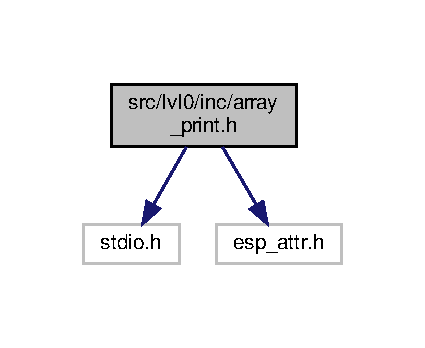
\includegraphics[width=269pt]{array__print_8h__incl}
\end{center}
\end{figure}
This graph shows which files directly or indirectly include this file\+:
\nopagebreak
\begin{figure}[H]
\begin{center}
\leavevmode
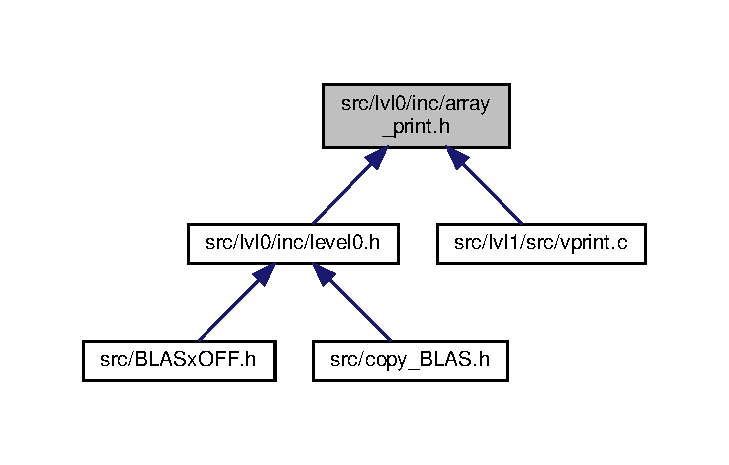
\includegraphics[width=284pt]{array__print_8h__dep__incl}
\end{center}
\end{figure}
\subsection*{Functions}
\begin{DoxyCompactItemize}
\item 
void I\+R\+A\+M\+\_\+\+A\+T\+TR \hyperlink{array__print_8h_a1452525829b0cf910e14b65121a0c53d}{array\+\_\+print} (char $\ast$string, const float $\ast$arr\+Src, const unsigned int start, const unsigned int end) \+\_\+\+\_\+attribute\+\_\+\+\_\+((always\+\_\+inline)) \+\_\+\+\_\+attribute\+\_\+\+\_\+((nonull))
\end{DoxyCompactItemize}


\subsection{Function Documentation}
\mbox{\Hypertarget{array__print_8h_a1452525829b0cf910e14b65121a0c53d}\label{array__print_8h_a1452525829b0cf910e14b65121a0c53d}} 
\index{array\+\_\+print.\+h@{array\+\_\+print.\+h}!array\+\_\+print@{array\+\_\+print}}
\index{array\+\_\+print@{array\+\_\+print}!array\+\_\+print.\+h@{array\+\_\+print.\+h}}
\subsubsection{\texorpdfstring{array\+\_\+print()}{array\_print()}}
{\footnotesize\ttfamily void I\+R\+A\+M\+\_\+\+A\+T\+TR array\+\_\+print (\begin{DoxyParamCaption}\item[{char $\ast$}]{string,  }\item[{const float $\ast$}]{arr\+Src,  }\item[{const unsigned int}]{start,  }\item[{const unsigned int}]{end }\end{DoxyParamCaption})}

Returns a pointer to a printable string of the data in a Vector 
\begin{DoxyParams}{Parameters}
{\em string} & Pointer to string buffer for printing \\
\hline
{\em arr\+Src} & Array pointer for source data \\
\hline
{\em start} & Starting element index to loop across \\
\hline
{\em end} & Last element index to loop across \\
\hline
\end{DoxyParams}

\hypertarget{array__puts_8h}{}\section{src/lvl0/inc/array\+\_\+puts.h File Reference}
\label{array__puts_8h}\index{src/lvl0/inc/array\+\_\+puts.\+h@{src/lvl0/inc/array\+\_\+puts.\+h}}
{\ttfamily \#include \char`\"{}esp\+\_\+attr.\+h\char`\"{}}\newline
{\ttfamily \#include \char`\"{}../src/array\+\_\+puts.\+c\char`\"{}}\newline
Include dependency graph for array\+\_\+puts.\+h\+:\nopagebreak
\begin{figure}[H]
\begin{center}
\leavevmode
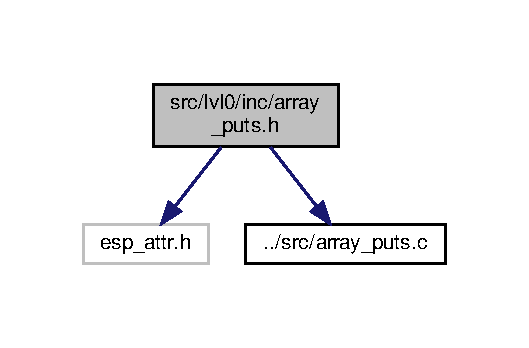
\includegraphics[width=254pt]{array__puts_8h__incl}
\end{center}
\end{figure}
This graph shows which files directly or indirectly include this file\+:
\nopagebreak
\begin{figure}[H]
\begin{center}
\leavevmode
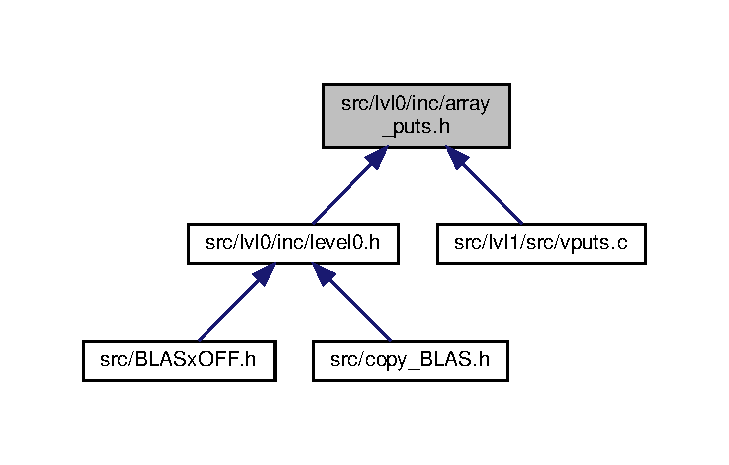
\includegraphics[width=284pt]{array__puts_8h__dep__incl}
\end{center}
\end{figure}
\subsection*{Functions}
\begin{DoxyCompactItemize}
\item 
void I\+R\+A\+M\+\_\+\+A\+T\+TR \hyperlink{array__puts_8h_a173a2544e1e54d9605348701522c160f}{array\+\_\+puts} (char $\ast$string, const float $\ast$arr\+Src, const unsigned int start, const unsigned int end) \+\_\+\+\_\+attribute\+\_\+\+\_\+((always\+\_\+inline)) \+\_\+\+\_\+attribute\+\_\+\+\_\+((nonull))
\end{DoxyCompactItemize}


\subsection{Function Documentation}
\mbox{\Hypertarget{array__puts_8h_a173a2544e1e54d9605348701522c160f}\label{array__puts_8h_a173a2544e1e54d9605348701522c160f}} 
\index{array\+\_\+puts.\+h@{array\+\_\+puts.\+h}!array\+\_\+puts@{array\+\_\+puts}}
\index{array\+\_\+puts@{array\+\_\+puts}!array\+\_\+puts.\+h@{array\+\_\+puts.\+h}}
\subsubsection{\texorpdfstring{array\+\_\+puts()}{array\_puts()}}
{\footnotesize\ttfamily void I\+R\+A\+M\+\_\+\+A\+T\+TR array\+\_\+puts (\begin{DoxyParamCaption}\item[{char $\ast$}]{string,  }\item[{const float $\ast$}]{arr\+Src,  }\item[{const unsigned int}]{start,  }\item[{const unsigned int}]{end }\end{DoxyParamCaption})}

Returns a pointer to a putsable string with the return character \textquotesingle{}~\newline
\textquotesingle{} 
\begin{DoxyParams}{Parameters}
{\em string} & Pointer to string buffer for printing \\
\hline
{\em arr\+Src} & Array pointer for source data \\
\hline
{\em start} & Starting element index to loop across \\
\hline
{\em end} & Last element index to loop across \\
\hline
\end{DoxyParams}

\hypertarget{array__set_8h}{}\section{src/lvl0/inc/array\+\_\+set.h File Reference}
\label{array__set_8h}\index{src/lvl0/inc/array\+\_\+set.\+h@{src/lvl0/inc/array\+\_\+set.\+h}}
{\ttfamily \#include \char`\"{}esp\+\_\+attr.\+h\char`\"{}}\newline
Include dependency graph for array\+\_\+set.\+h\+:
\nopagebreak
\begin{figure}[H]
\begin{center}
\leavevmode
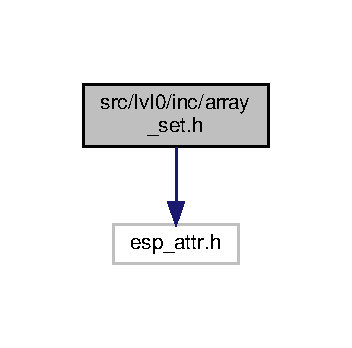
\includegraphics[width=169pt]{array__set_8h__incl}
\end{center}
\end{figure}
This graph shows which files directly or indirectly include this file\+:
\nopagebreak
\begin{figure}[H]
\begin{center}
\leavevmode
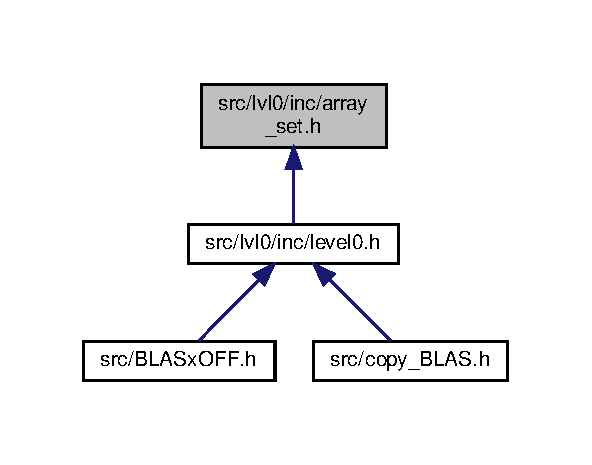
\includegraphics[width=284pt]{array__set_8h__dep__incl}
\end{center}
\end{figure}
\subsection*{Functions}
\begin{DoxyCompactItemize}
\item 
void I\+R\+A\+M\+\_\+\+A\+T\+TR \hyperlink{array__set_8h_a3f568bfbd4fde500e67a7d1ea14a114f}{\+\_\+\+\_\+attribute\+\_\+\+\_\+} ((always\+\_\+inline)) \+\_\+\+\_\+attribute\+\_\+\+\_\+((nonull))
\item 
\hyperlink{array__set_8h_a4783e2ea7e94e79636384acc4c542684}{array\+\_\+set} (float $\ast$arr\+Dst, const float \hyperlink{array__print_8h_a476893ee338bd7d79f15687de2dd39b2}{scl\+Src}, const unsigned int \hyperlink{array__zero_8h_a1951879481f1ba4287d30b0a485429fc}{start}, const unsigned int \hyperlink{array__zero_8h_ae062d39ef5523e038e43c08fa9fe07b4}{end})
\end{DoxyCompactItemize}


\subsection{Function Documentation}
\mbox{\Hypertarget{array__set_8h_a3f568bfbd4fde500e67a7d1ea14a114f}\label{array__set_8h_a3f568bfbd4fde500e67a7d1ea14a114f}} 
\index{array\+\_\+set.\+h@{array\+\_\+set.\+h}!\+\_\+\+\_\+attribute\+\_\+\+\_\+@{\+\_\+\+\_\+attribute\+\_\+\+\_\+}}
\index{\+\_\+\+\_\+attribute\+\_\+\+\_\+@{\+\_\+\+\_\+attribute\+\_\+\+\_\+}!array\+\_\+set.\+h@{array\+\_\+set.\+h}}
\subsubsection{\texorpdfstring{\+\_\+\+\_\+attribute\+\_\+\+\_\+()}{\_\_attribute\_\_()}}
{\footnotesize\ttfamily void I\+R\+A\+M\+\_\+\+A\+T\+TR \+\_\+\+\_\+attribute\+\_\+\+\_\+ (\begin{DoxyParamCaption}\item[{(always\+\_\+inline)}]{ }\end{DoxyParamCaption})\hspace{0.3cm}{\ttfamily [inline]}}

This function set two arrays together element by element

This function add two arrays together element by element

This function adds a scalar too each element in an array


\begin{DoxyItemize}
\item This function is deliberatly placed in Instruction R\+AM. Meaning that this function will always remained cached.
\item the {\bfseries attribute}((always\+\_\+inline)) tells the compiler to A\+L\+W\+A\+YS inline to function reguardless of optimization levels
\item the {\bfseries attribute}((nonull)) tells the compiler that the function\textquotesingle{}s pointer arguments cannot bell N\+U\+LL
\end{DoxyItemize}

This function adds all the elements in an array and returns the sum

This function copies the elements of one arrays into another array

This function computes the dot product between two arrays

This function multiplies each element of an array by a scalar

This function multiplies elements of an array by a scalar

This function Zeros the elements in an array \mbox{\Hypertarget{array__set_8h_a4783e2ea7e94e79636384acc4c542684}\label{array__set_8h_a4783e2ea7e94e79636384acc4c542684}} 
\index{array\+\_\+set.\+h@{array\+\_\+set.\+h}!array\+\_\+set@{array\+\_\+set}}
\index{array\+\_\+set@{array\+\_\+set}!array\+\_\+set.\+h@{array\+\_\+set.\+h}}
\subsubsection{\texorpdfstring{array\+\_\+set()}{array\_set()}}
{\footnotesize\ttfamily array\+\_\+set (\begin{DoxyParamCaption}\item[{float $\ast$}]{arr\+Dst,  }\item[{const float}]{scl\+Src,  }\item[{const unsigned int}]{start,  }\item[{const unsigned int}]{end }\end{DoxyParamCaption})}


\begin{DoxyParams}{Parameters}
{\em arr\+Dst} & Array pointer where the result will be stored \\
\hline
{\em scl\+Src} & Float for the source scalar \\
\hline
{\em start} & Starting element index to loop across \\
\hline
{\em end} & Last element index to loop across \\
\hline
\end{DoxyParams}

\hypertarget{array__subtract_8h}{}\section{src/lvl0/inc/array\+\_\+subtract.h File Reference}
\label{array__subtract_8h}\index{src/lvl0/inc/array\+\_\+subtract.\+h@{src/lvl0/inc/array\+\_\+subtract.\+h}}
{\ttfamily \#include \char`\"{}esp\+\_\+attr.\+h\char`\"{}}\newline
Include dependency graph for array\+\_\+subtract.\+h\+:
\nopagebreak
\begin{figure}[H]
\begin{center}
\leavevmode
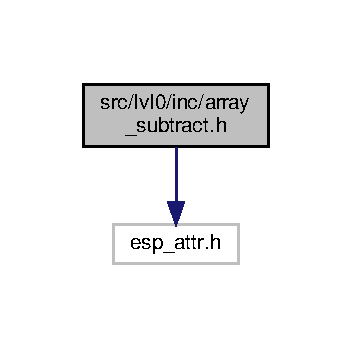
\includegraphics[width=169pt]{array__subtract_8h__incl}
\end{center}
\end{figure}
This graph shows which files directly or indirectly include this file\+:
\nopagebreak
\begin{figure}[H]
\begin{center}
\leavevmode
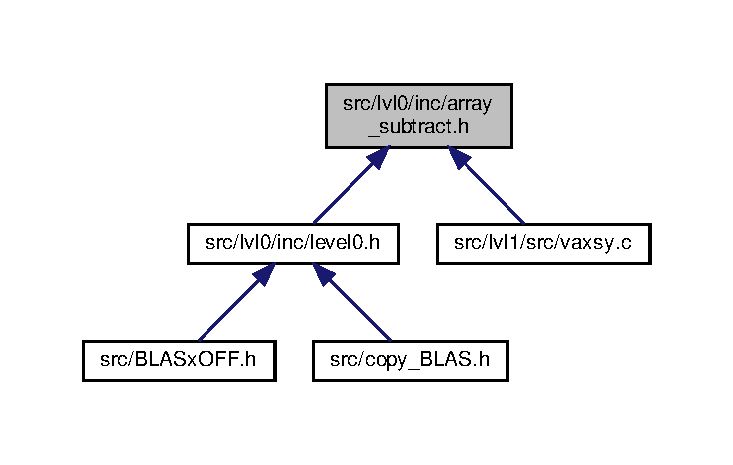
\includegraphics[width=350pt]{array__subtract_8h__dep__incl}
\end{center}
\end{figure}
\subsection*{Functions}
\begin{DoxyCompactItemize}
\item 
void I\+R\+A\+M\+\_\+\+A\+T\+TR \hyperlink{array__subtract_8h_a33d9ae6a3856a1da4409e370ff6f24f8}{\+\_\+\+\_\+attribute\+\_\+\+\_\+} ((always\+\_\+inline)) \+\_\+\+\_\+attribute\+\_\+\+\_\+((nonull)) array\+\_\+substract(float $\ast$arr\+Res
\end{DoxyCompactItemize}
\subsection*{Variables}
\begin{DoxyCompactItemize}
\item 
void I\+R\+A\+M\+\_\+\+A\+T\+TR const float $\ast$ \hyperlink{array__subtract_8h_a5e4e071457fdcdd98fd22e75c6bfc555}{arr\+OprA}
\begin{DoxyCompactList}\small\item\em $<$ Array pointer where the result will be stored \end{DoxyCompactList}\item 
void I\+R\+A\+M\+\_\+\+A\+T\+TR const float const float $\ast$ \hyperlink{array__subtract_8h_ad0fdcae3b6e2275dc980d15e3726a6a1}{arr\+OprB}
\begin{DoxyCompactList}\small\item\em Array pointer for the 2nd operand. \end{DoxyCompactList}\item 
void I\+R\+A\+M\+\_\+\+A\+T\+TR const float const float const unsigned int \hyperlink{array__subtract_8h_a0549b2187026de7f72c6b3214fa437d5}{start}
\begin{DoxyCompactList}\small\item\em Starting element index to loop across. \end{DoxyCompactList}\item 
void I\+R\+A\+M\+\_\+\+A\+T\+TR const float const float const unsigned int const unsigned int \hyperlink{array__subtract_8h_a68c28899964e31626b3c9e42853f0d42}{end}
\begin{DoxyCompactList}\small\item\em $<$ Last element index to loop across \end{DoxyCompactList}\end{DoxyCompactItemize}


\subsection{Function Documentation}
\mbox{\Hypertarget{array__subtract_8h_a33d9ae6a3856a1da4409e370ff6f24f8}\label{array__subtract_8h_a33d9ae6a3856a1da4409e370ff6f24f8}} 
\index{array\+\_\+subtract.\+h@{array\+\_\+subtract.\+h}!\+\_\+\+\_\+attribute\+\_\+\+\_\+@{\+\_\+\+\_\+attribute\+\_\+\+\_\+}}
\index{\+\_\+\+\_\+attribute\+\_\+\+\_\+@{\+\_\+\+\_\+attribute\+\_\+\+\_\+}!array\+\_\+subtract.\+h@{array\+\_\+subtract.\+h}}
\subsubsection{\texorpdfstring{\+\_\+\+\_\+attribute\+\_\+\+\_\+()}{\_\_attribute\_\_()}}
{\footnotesize\ttfamily void I\+R\+A\+M\+\_\+\+A\+T\+TR \+\_\+\+\_\+attribute\+\_\+\+\_\+ (\begin{DoxyParamCaption}\item[{(always\+\_\+inline)}]{ }\end{DoxyParamCaption})}

This function substract two arrays together element by element 

\subsection{Variable Documentation}
\mbox{\Hypertarget{array__subtract_8h_a5e4e071457fdcdd98fd22e75c6bfc555}\label{array__subtract_8h_a5e4e071457fdcdd98fd22e75c6bfc555}} 
\index{array\+\_\+subtract.\+h@{array\+\_\+subtract.\+h}!arr\+OprA@{arr\+OprA}}
\index{arr\+OprA@{arr\+OprA}!array\+\_\+subtract.\+h@{array\+\_\+subtract.\+h}}
\subsubsection{\texorpdfstring{arr\+OprA}{arrOprA}}
{\footnotesize\ttfamily void I\+R\+A\+M\+\_\+\+A\+T\+TR const float$\ast$ arr\+OprA}



$<$ Array pointer where the result will be stored 

Array pointer for the 1st operand \mbox{\Hypertarget{array__subtract_8h_ad0fdcae3b6e2275dc980d15e3726a6a1}\label{array__subtract_8h_ad0fdcae3b6e2275dc980d15e3726a6a1}} 
\index{array\+\_\+subtract.\+h@{array\+\_\+subtract.\+h}!arr\+OprB@{arr\+OprB}}
\index{arr\+OprB@{arr\+OprB}!array\+\_\+subtract.\+h@{array\+\_\+subtract.\+h}}
\subsubsection{\texorpdfstring{arr\+OprB}{arrOprB}}
{\footnotesize\ttfamily void I\+R\+A\+M\+\_\+\+A\+T\+TR const float const float$\ast$ arr\+OprB}



Array pointer for the 2nd operand. 

\mbox{\Hypertarget{array__subtract_8h_a68c28899964e31626b3c9e42853f0d42}\label{array__subtract_8h_a68c28899964e31626b3c9e42853f0d42}} 
\index{array\+\_\+subtract.\+h@{array\+\_\+subtract.\+h}!end@{end}}
\index{end@{end}!array\+\_\+subtract.\+h@{array\+\_\+subtract.\+h}}
\subsubsection{\texorpdfstring{end}{end}}
{\footnotesize\ttfamily void I\+R\+A\+M\+\_\+\+A\+T\+TR const float const float const unsigned int const unsigned int end}

{\bfseries Initial value\+:}
\begin{DoxyCode}
\{
    \textcolor{keywordflow}{for}(\textcolor{keywordtype}{unsigned} \textcolor{keywordtype}{int} I=\hyperlink{array__subtract_8h_a0549b2187026de7f72c6b3214fa437d5}{start}; I<\hyperlink{array__subtract_8h_a68c28899964e31626b3c9e42853f0d42}{end}; ++I) \{
      arrRes[I] = \hyperlink{array__subtract_8h_a5e4e071457fdcdd98fd22e75c6bfc555}{arrOprA} - \hyperlink{array__subtract_8h_ad0fdcae3b6e2275dc980d15e3726a6a1}{arrOprB};
    \}
    \textcolor{keywordflow}{return}
\end{DoxyCode}


$<$ Last element index to loop across 

\mbox{\Hypertarget{array__subtract_8h_a0549b2187026de7f72c6b3214fa437d5}\label{array__subtract_8h_a0549b2187026de7f72c6b3214fa437d5}} 
\index{array\+\_\+subtract.\+h@{array\+\_\+subtract.\+h}!start@{start}}
\index{start@{start}!array\+\_\+subtract.\+h@{array\+\_\+subtract.\+h}}
\subsubsection{\texorpdfstring{start}{start}}
{\footnotesize\ttfamily void I\+R\+A\+M\+\_\+\+A\+T\+TR const float const float const unsigned int start}



Starting element index to loop across. 


\hypertarget{array__swap_8h}{}\section{src/lvl0/inc/array\+\_\+swap.h File Reference}
\label{array__swap_8h}\index{src/lvl0/inc/array\+\_\+swap.\+h@{src/lvl0/inc/array\+\_\+swap.\+h}}
{\ttfamily \#include \char`\"{}esp\+\_\+attr.\+h\char`\"{}}\newline
Include dependency graph for array\+\_\+swap.\+h\+:
\nopagebreak
\begin{figure}[H]
\begin{center}
\leavevmode
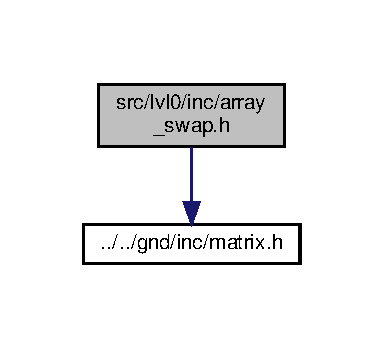
\includegraphics[width=169pt]{array__swap_8h__incl}
\end{center}
\end{figure}
This graph shows which files directly or indirectly include this file\+:\nopagebreak
\begin{figure}[H]
\begin{center}
\leavevmode
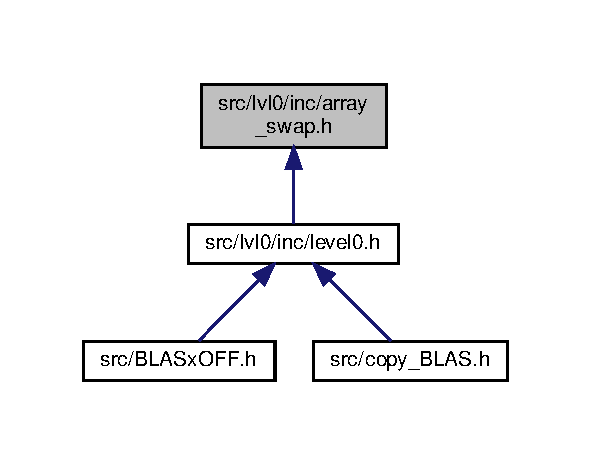
\includegraphics[width=284pt]{array__swap_8h__dep__incl}
\end{center}
\end{figure}
\subsection*{Functions}
\begin{DoxyCompactItemize}
\item 
void I\+R\+A\+M\+\_\+\+A\+T\+TR \hyperlink{array__swap_8h_ac2e028e05235dd050c3da6f604ae22fd}{\+\_\+\+\_\+attribute\+\_\+\+\_\+} ((always\+\_\+inline)) \+\_\+\+\_\+attribute\+\_\+\+\_\+((nonull)) array\+\_\+swap(float $\ast$\hyperlink{array__swap_8h_afbf35f33b730696364a33663ecc97c06}{arr\+Src\+DstA}
\end{DoxyCompactItemize}
\subsection*{Variables}
\begin{DoxyCompactItemize}
\item 
void I\+R\+A\+M\+\_\+\+A\+T\+TR float $\ast$ \hyperlink{array__swap_8h_a4916c4f9ec623c8a595e3282283c2c4c}{arr\+Src\+DstB}
\item 
\hyperlink{array__swap_8h_afbf35f33b730696364a33663ecc97c06}{arr\+Src\+DstA} = \hyperlink{array__swap_8h_a4916c4f9ec623c8a595e3282283c2c4c}{arr\+Src\+DstB}
\item 
\hyperlink{array__swap_8h_a9717e7bbecb906637e86cef6da3d83c2}{return}
\end{DoxyCompactItemize}


\subsection{Function Documentation}
\mbox{\Hypertarget{array__swap_8h_ac2e028e05235dd050c3da6f604ae22fd}\label{array__swap_8h_ac2e028e05235dd050c3da6f604ae22fd}} 
\index{array\+\_\+swap.\+h@{array\+\_\+swap.\+h}!\+\_\+\+\_\+attribute\+\_\+\+\_\+@{\+\_\+\+\_\+attribute\+\_\+\+\_\+}}
\index{\+\_\+\+\_\+attribute\+\_\+\+\_\+@{\+\_\+\+\_\+attribute\+\_\+\+\_\+}!array\+\_\+swap.\+h@{array\+\_\+swap.\+h}}
\subsubsection{\texorpdfstring{\+\_\+\+\_\+attribute\+\_\+\+\_\+()}{\_\_attribute\_\_()}}
{\footnotesize\ttfamily void I\+R\+A\+M\+\_\+\+A\+T\+TR \+\_\+\+\_\+attribute\+\_\+\+\_\+ (\begin{DoxyParamCaption}\item[{(always\+\_\+inline)}]{ }\end{DoxyParamCaption})}

This function swap two arrays together element by element 

\subsection{Variable Documentation}
\mbox{\Hypertarget{array__swap_8h_afbf35f33b730696364a33663ecc97c06}\label{array__swap_8h_afbf35f33b730696364a33663ecc97c06}} 
\index{array\+\_\+swap.\+h@{array\+\_\+swap.\+h}!arr\+Src\+DstA@{arr\+Src\+DstA}}
\index{arr\+Src\+DstA@{arr\+Src\+DstA}!array\+\_\+swap.\+h@{array\+\_\+swap.\+h}}
\subsubsection{\texorpdfstring{arr\+Src\+DstA}{arrSrcDstA}}
{\footnotesize\ttfamily arr\+Src\+DstA = \hyperlink{array__swap_8h_a4916c4f9ec623c8a595e3282283c2c4c}{arr\+Src\+DstB}}

\mbox{\Hypertarget{array__swap_8h_a4916c4f9ec623c8a595e3282283c2c4c}\label{array__swap_8h_a4916c4f9ec623c8a595e3282283c2c4c}} 
\index{array\+\_\+swap.\+h@{array\+\_\+swap.\+h}!arr\+Src\+DstB@{arr\+Src\+DstB}}
\index{arr\+Src\+DstB@{arr\+Src\+DstB}!array\+\_\+swap.\+h@{array\+\_\+swap.\+h}}
\subsubsection{\texorpdfstring{arr\+Src\+DstB}{arrSrcDstB}}
{\footnotesize\ttfamily arr\+Src\+DstB}

{\bfseries Initial value\+:}
\begin{DoxyCode}
\{
    \textcolor{keywordtype}{float} * temp = \hyperlink{array__swap_8h_afbf35f33b730696364a33663ecc97c06}{arrSrcDstA}
\end{DoxyCode}
\mbox{\Hypertarget{array__swap_8h_a9717e7bbecb906637e86cef6da3d83c2}\label{array__swap_8h_a9717e7bbecb906637e86cef6da3d83c2}} 
\index{array\+\_\+swap.\+h@{array\+\_\+swap.\+h}!return@{return}}
\index{return@{return}!array\+\_\+swap.\+h@{array\+\_\+swap.\+h}}
\subsubsection{\texorpdfstring{return}{return}}
{\footnotesize\ttfamily return}


\hypertarget{array__zero_8h}{}\section{src/lvl0/inc/array\+\_\+zero.h File Reference}
\label{array__zero_8h}\index{src/lvl0/inc/array\+\_\+zero.\+h@{src/lvl0/inc/array\+\_\+zero.\+h}}
{\ttfamily \#include \char`\"{}esp\+\_\+attr.\+h\char`\"{}}\newline
{\ttfamily \#include \char`\"{}../src/array\+\_\+zero.\+c\+\_\+\+\_\+\char`\"{}}\newline
Include dependency graph for array\+\_\+zero.\+h\+:
\nopagebreak
\begin{figure}[H]
\begin{center}
\leavevmode
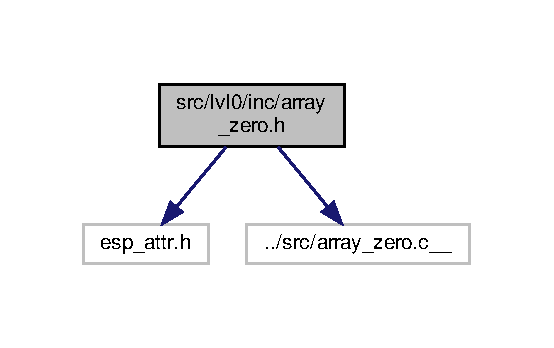
\includegraphics[width=266pt]{array__zero_8h__incl}
\end{center}
\end{figure}
This graph shows which files directly or indirectly include this file\+:\nopagebreak
\begin{figure}[H]
\begin{center}
\leavevmode
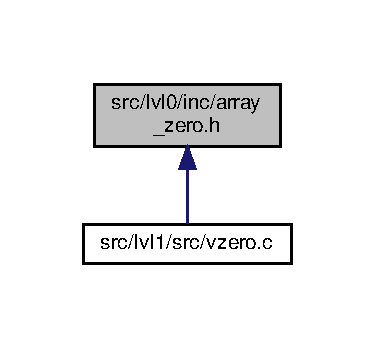
\includegraphics[width=180pt]{array__zero_8h__dep__incl}
\end{center}
\end{figure}
\subsection*{Functions}
\begin{DoxyCompactItemize}
\item 
void I\+R\+A\+M\+\_\+\+A\+T\+TR \hyperlink{array__zero_8h_a56e0537cf29dc30e0320a18e290caa5b}{array\+\_\+zero} (float $\ast$arr\+Dst, const unsigned int start, const unsigned int end) \+\_\+\+\_\+attribute\+\_\+\+\_\+((always\+\_\+inline)) \+\_\+\+\_\+attribute\+\_\+\+\_\+((nonull))
\end{DoxyCompactItemize}


\subsection{Function Documentation}
\mbox{\Hypertarget{array__zero_8h_a56e0537cf29dc30e0320a18e290caa5b}\label{array__zero_8h_a56e0537cf29dc30e0320a18e290caa5b}} 
\index{array\+\_\+zero.\+h@{array\+\_\+zero.\+h}!array\+\_\+zero@{array\+\_\+zero}}
\index{array\+\_\+zero@{array\+\_\+zero}!array\+\_\+zero.\+h@{array\+\_\+zero.\+h}}
\subsubsection{\texorpdfstring{array\+\_\+zero()}{array\_zero()}}
{\footnotesize\ttfamily void I\+R\+A\+M\+\_\+\+A\+T\+TR array\+\_\+zero (\begin{DoxyParamCaption}\item[{float $\ast$}]{arr\+Dst,  }\item[{const unsigned int}]{start,  }\item[{const unsigned int}]{end }\end{DoxyParamCaption})}

This function Zeros the elements in an array 
\begin{DoxyParams}{Parameters}
{\em arr\+Dst} & Array pointer where the result will be stored \\
\hline
{\em start} & Starting element index to loop across \\
\hline
{\em end} & Last element index to loop across \\
\hline
\end{DoxyParams}
Here is the caller graph for this function\+:\nopagebreak
\begin{figure}[H]
\begin{center}
\leavevmode
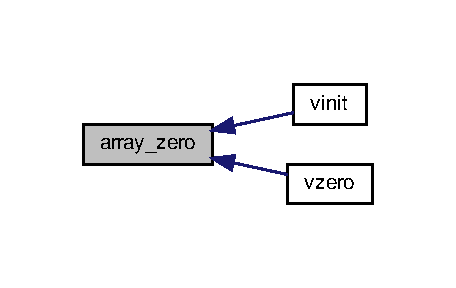
\includegraphics[width=219pt]{array__zero_8h_a56e0537cf29dc30e0320a18e290caa5b_icgraph}
\end{center}
\end{figure}

\hypertarget{level0_8h}{}\section{src/lvl0/inc/level0.h File Reference}
\label{level0_8h}\index{src/lvl0/inc/level0.\+h@{src/lvl0/inc/level0.\+h}}
{\ttfamily \#include \char`\"{}array\+\_\+add.\+h\char`\"{}}\newline
{\ttfamily \#include \char`\"{}array\+\_\+ascl.\+h\char`\"{}}\newline
{\ttfamily \#include \char`\"{}array\+\_\+asum.\+h\char`\"{}}\newline
{\ttfamily \#include \char`\"{}array\+\_\+copy.\+h\char`\"{}}\newline
{\ttfamily \#include \char`\"{}array\+\_\+dot.\+h\char`\"{}}\newline
{\ttfamily \#include \char`\"{}array\+\_\+mscl.\+h\char`\"{}}\newline
{\ttfamily \#include \char`\"{}array\+\_\+mult.\+h\char`\"{}}\newline
{\ttfamily \#include \char`\"{}array\+\_\+print.\+h\char`\"{}}\newline
{\ttfamily \#include \char`\"{}array\+\_\+puts.\+h\char`\"{}}\newline
{\ttfamily \#include \char`\"{}array\+\_\+set.\+h\char`\"{}}\newline
{\ttfamily \#include \char`\"{}array\+\_\+subtract.\+h\char`\"{}}\newline
{\ttfamily \#include \char`\"{}array\+\_\+swap.\+h\char`\"{}}\newline
Include dependency graph for level0.\+h\+:
\nopagebreak
\begin{figure}[H]
\begin{center}
\leavevmode
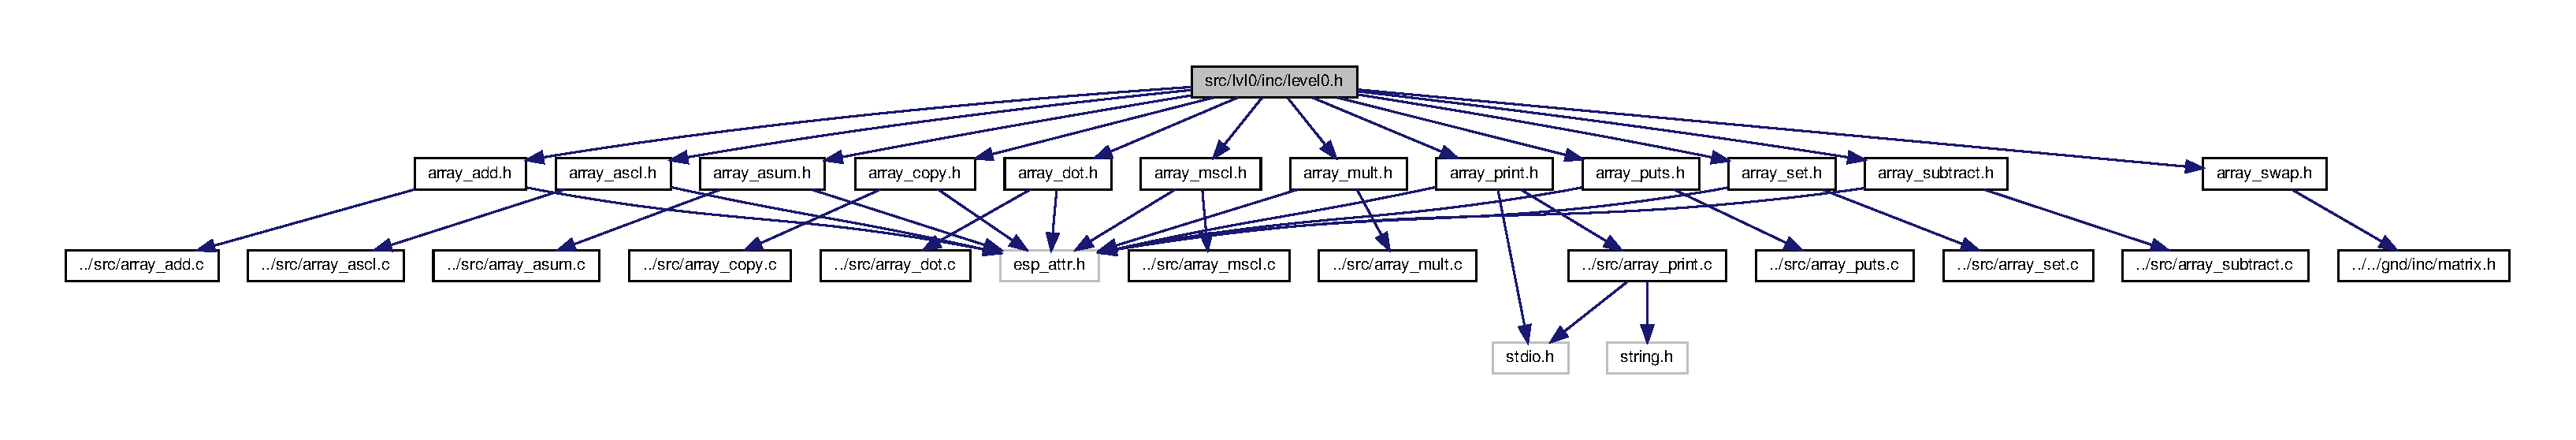
\includegraphics[width=350pt]{level0_8h__incl}
\end{center}
\end{figure}
This graph shows which files directly or indirectly include this file\+:
\nopagebreak
\begin{figure}[H]
\begin{center}
\leavevmode
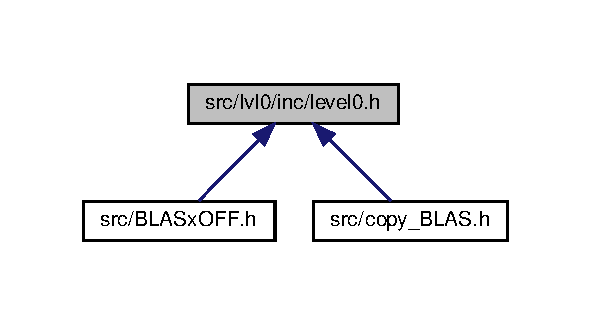
\includegraphics[width=284pt]{level0_8h__dep__incl}
\end{center}
\end{figure}

\hypertarget{array__add_8c}{}\section{src/lvl0/src/array\+\_\+add.c File Reference}
\label{array__add_8c}\index{src/lvl0/src/array\+\_\+add.\+c@{src/lvl0/src/array\+\_\+add.\+c}}
\subsection*{Functions}
\begin{DoxyCompactItemize}
\item 
void \hyperlink{array__add_8c_a6187039d26693e108051c0484d4794de}{array\+\_\+add} (float $\ast$arr\+Res, const float $\ast$arr\+OprA, const float $\ast$arr\+OprB, const unsigned int start, const unsigned int end)
\end{DoxyCompactItemize}


\subsection{Function Documentation}
\mbox{\Hypertarget{array__add_8c_a6187039d26693e108051c0484d4794de}\label{array__add_8c_a6187039d26693e108051c0484d4794de}} 
\index{array\+\_\+add.\+c@{array\+\_\+add.\+c}!array\+\_\+add@{array\+\_\+add}}
\index{array\+\_\+add@{array\+\_\+add}!array\+\_\+add.\+c@{array\+\_\+add.\+c}}
\subsubsection{\texorpdfstring{array\+\_\+add()}{array\_add()}}
{\footnotesize\ttfamily void array\+\_\+add (\begin{DoxyParamCaption}\item[{float $\ast$}]{arr\+Res,  }\item[{const float $\ast$}]{arr\+OprA,  }\item[{const float $\ast$}]{arr\+OprB,  }\item[{const unsigned int}]{start,  }\item[{const unsigned int}]{end }\end{DoxyParamCaption})}

This function add two arrays together element by element 
\begin{DoxyParams}{Parameters}
{\em arr\+Res} & Array pointer where the result will be stored \\
\hline
{\em arr\+OprA} & Array pointer for the 1st operand \\
\hline
{\em arr\+OprB} & Array pointer for the 2nd operand \\
\hline
{\em start} & Starting element index to loop across \\
\hline
{\em end} & Last element index to loop across \\
\hline
\end{DoxyParams}
Here is the caller graph for this function\+:
\nopagebreak
\begin{figure}[H]
\begin{center}
\leavevmode
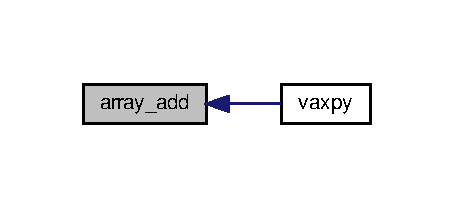
\includegraphics[width=218pt]{array__add_8c_a6187039d26693e108051c0484d4794de_icgraph}
\end{center}
\end{figure}

\hypertarget{array__ascl_8c}{}\section{src/lvl0/src/array\+\_\+ascl.c File Reference}
\label{array__ascl_8c}\index{src/lvl0/src/array\+\_\+ascl.\+c@{src/lvl0/src/array\+\_\+ascl.\+c}}
This graph shows which files directly or indirectly include this file\+:
\nopagebreak
\begin{figure}[H]
\begin{center}
\leavevmode
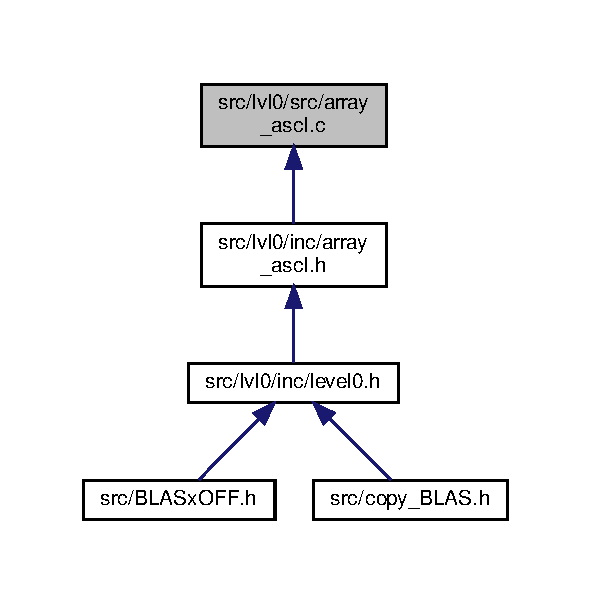
\includegraphics[width=349pt]{array__ascl_8c__dep__incl}
\end{center}
\end{figure}
\subsection*{Functions}
\begin{DoxyCompactItemize}
\item 
void \hyperlink{array__ascl_8c_a1b7fb9cb6e0e56609c457c914f9548d4}{array\+\_\+ascl} (float $\ast$arr\+Res, const float $\ast$arr\+Opr, const float scl\+Opr, const unsigned int start, const unsigned int end)
\end{DoxyCompactItemize}


\subsection{Function Documentation}
\mbox{\Hypertarget{array__ascl_8c_a1b7fb9cb6e0e56609c457c914f9548d4}\label{array__ascl_8c_a1b7fb9cb6e0e56609c457c914f9548d4}} 
\index{array\+\_\+ascl.\+c@{array\+\_\+ascl.\+c}!array\+\_\+ascl@{array\+\_\+ascl}}
\index{array\+\_\+ascl@{array\+\_\+ascl}!array\+\_\+ascl.\+c@{array\+\_\+ascl.\+c}}
\subsubsection{\texorpdfstring{array\+\_\+ascl()}{array\_ascl()}}
{\footnotesize\ttfamily void array\+\_\+ascl (\begin{DoxyParamCaption}\item[{float $\ast$}]{arr\+Res,  }\item[{const float $\ast$}]{arr\+Opr,  }\item[{const float}]{scl\+Opr,  }\item[{const unsigned int}]{start,  }\item[{const unsigned int}]{end }\end{DoxyParamCaption})}

Function definition for adding a scalar to an array 
\begin{DoxyParams}{Parameters}
{\em arr\+Res} & Array pointer where the result will be stored \\
\hline
{\em arr\+Opr} & Pointer for the array operand \\
\hline
{\em scl\+Opr} & Scalar operand to add to the elements of the array operand \\
\hline
{\em start} & Begining element index to begin loop \\
\hline
{\em end} & Last element index to loop across \\
\hline
\end{DoxyParams}
Here is the caller graph for this function\+:
\nopagebreak
\begin{figure}[H]
\begin{center}
\leavevmode
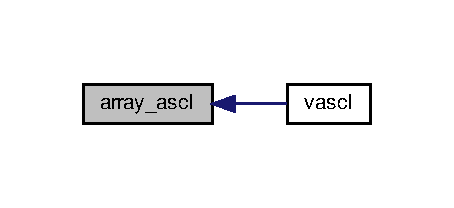
\includegraphics[width=218pt]{array__ascl_8c_a1b7fb9cb6e0e56609c457c914f9548d4_icgraph}
\end{center}
\end{figure}

\hypertarget{array__asum_8c}{}\section{src/lvl0/src/array\+\_\+asum.c File Reference}
\label{array__asum_8c}\index{src/lvl0/src/array\+\_\+asum.\+c@{src/lvl0/src/array\+\_\+asum.\+c}}
This graph shows which files directly or indirectly include this file\+:
\nopagebreak
\begin{figure}[H]
\begin{center}
\leavevmode
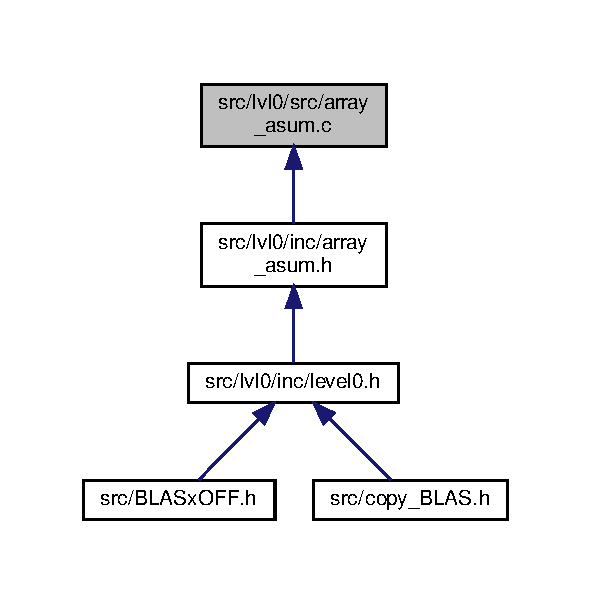
\includegraphics[width=350pt]{array__asum_8c__dep__incl}
\end{center}
\end{figure}
\subsection*{Functions}
\begin{DoxyCompactItemize}
\item 
void \hyperlink{array__asum_8c_a9278eb0e573f6e18263911caa6818e44}{array\+\_\+asum} (float $\ast$scl\+Res, const float $\ast$arr\+Opr, const unsigned int start, const unsigned int end)
\end{DoxyCompactItemize}


\subsection{Function Documentation}
\mbox{\Hypertarget{array__asum_8c_a9278eb0e573f6e18263911caa6818e44}\label{array__asum_8c_a9278eb0e573f6e18263911caa6818e44}} 
\index{array\+\_\+asum.\+c@{array\+\_\+asum.\+c}!array\+\_\+asum@{array\+\_\+asum}}
\index{array\+\_\+asum@{array\+\_\+asum}!array\+\_\+asum.\+c@{array\+\_\+asum.\+c}}
\subsubsection{\texorpdfstring{array\+\_\+asum()}{array\_asum()}}
{\footnotesize\ttfamily void array\+\_\+asum (\begin{DoxyParamCaption}\item[{float $\ast$}]{scl\+Res,  }\item[{const float $\ast$}]{arr\+Opr,  }\item[{const unsigned int}]{start,  }\item[{const unsigned int}]{end }\end{DoxyParamCaption})}

This function adds all the elements in an array and returns the sum 
\begin{DoxyParams}{Parameters}
{\em scl\+Res} & Float pointer for return value \\
\hline
{\em arr\+Opr} & Array pointer for elements to sum \\
\hline
{\em start} & Starting element index to loop across \\
\hline
{\em end} & Last element index to loop across \\
\hline
\end{DoxyParams}
Here is the caller graph for this function\+:
\nopagebreak
\begin{figure}[H]
\begin{center}
\leavevmode
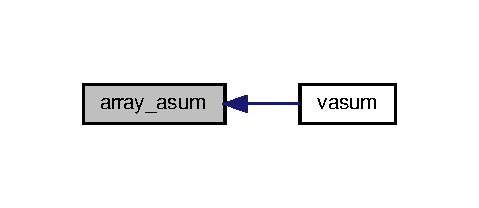
\includegraphics[width=230pt]{array__asum_8c_a9278eb0e573f6e18263911caa6818e44_icgraph}
\end{center}
\end{figure}

\hypertarget{array__copy_8c}{}\section{src/lvl0/src/array\+\_\+copy.c File Reference}
\label{array__copy_8c}\index{src/lvl0/src/array\+\_\+copy.\+c@{src/lvl0/src/array\+\_\+copy.\+c}}
This graph shows which files directly or indirectly include this file\+:
\nopagebreak
\begin{figure}[H]
\begin{center}
\leavevmode
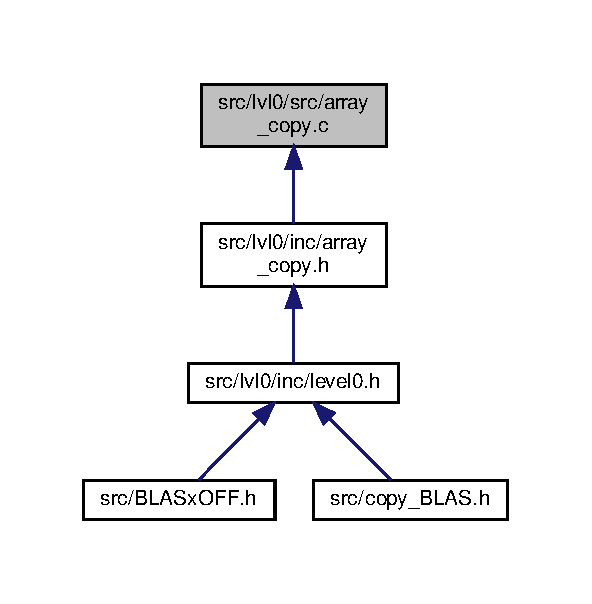
\includegraphics[width=350pt]{array__copy_8c__dep__incl}
\end{center}
\end{figure}
\subsection*{Functions}
\begin{DoxyCompactItemize}
\item 
void \hyperlink{array__copy_8c_a474f406afeffe18d675d3fd858d03fd3}{array\+\_\+copy} (float $\ast$arr\+Dst, const float $\ast$arr\+Src, const unsigned int start, const unsigned int end)
\end{DoxyCompactItemize}


\subsection{Function Documentation}
\mbox{\Hypertarget{array__copy_8c_a474f406afeffe18d675d3fd858d03fd3}\label{array__copy_8c_a474f406afeffe18d675d3fd858d03fd3}} 
\index{array\+\_\+copy.\+c@{array\+\_\+copy.\+c}!array\+\_\+copy@{array\+\_\+copy}}
\index{array\+\_\+copy@{array\+\_\+copy}!array\+\_\+copy.\+c@{array\+\_\+copy.\+c}}
\subsubsection{\texorpdfstring{array\+\_\+copy()}{array\_copy()}}
{\footnotesize\ttfamily void array\+\_\+copy (\begin{DoxyParamCaption}\item[{float $\ast$}]{arr\+Dst,  }\item[{const float $\ast$}]{arr\+Src,  }\item[{const unsigned int}]{start,  }\item[{const unsigned int}]{end }\end{DoxyParamCaption})}

This function copies the elements of one arrays into another array 
\begin{DoxyParams}{Parameters}
{\em arr\+Dst} & Array pointer destination to copy source data into \\
\hline
{\em arr\+Src} & Array pointer for source data \\
\hline
{\em start} & Starting element index to loop across \\
\hline
{\em end} & Last element index to loop across \\
\hline
\end{DoxyParams}
Here is the caller graph for this function\+:
\nopagebreak
\begin{figure}[H]
\begin{center}
\leavevmode
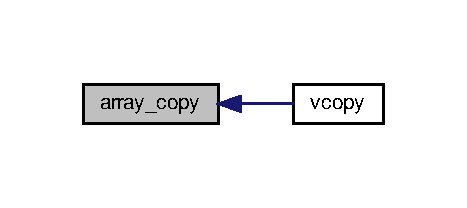
\includegraphics[width=224pt]{array__copy_8c_a474f406afeffe18d675d3fd858d03fd3_icgraph}
\end{center}
\end{figure}

\hypertarget{array__dot_8c}{}\section{src/lvl0/src/array\+\_\+dot.c File Reference}
\label{array__dot_8c}\index{src/lvl0/src/array\+\_\+dot.\+c@{src/lvl0/src/array\+\_\+dot.\+c}}
\subsection*{Functions}
\begin{DoxyCompactItemize}
\item 
void \hyperlink{array__dot_8c_ac4f56b27723842c5a133d553096e1483}{array\+\_\+dot} (float $\ast$scl\+Res, const float $\ast$arr\+OprA, const float $\ast$arr\+OprB, const unsigned int start, const unsigned int end)
\end{DoxyCompactItemize}


\subsection{Function Documentation}
\mbox{\Hypertarget{array__dot_8c_ac4f56b27723842c5a133d553096e1483}\label{array__dot_8c_ac4f56b27723842c5a133d553096e1483}} 
\index{array\+\_\+dot.\+c@{array\+\_\+dot.\+c}!array\+\_\+dot@{array\+\_\+dot}}
\index{array\+\_\+dot@{array\+\_\+dot}!array\+\_\+dot.\+c@{array\+\_\+dot.\+c}}
\subsubsection{\texorpdfstring{array\+\_\+dot()}{array\_dot()}}
{\footnotesize\ttfamily void array\+\_\+dot (\begin{DoxyParamCaption}\item[{float $\ast$}]{scl\+Res,  }\item[{const float $\ast$}]{arr\+OprA,  }\item[{const float $\ast$}]{arr\+OprB,  }\item[{const unsigned int}]{start,  }\item[{const unsigned int}]{end }\end{DoxyParamCaption})}

This function computes the dot product between two arrays 
\begin{DoxyParams}{Parameters}
{\em scl\+Res} & Array pointer where the result will be stored \\
\hline
{\em arr\+OprA} & Array pointer for the 1st operand \\
\hline
{\em arr\+OprB} & Array pointer for the 2nd operand \\
\hline
{\em start} & Starting element index to loop across \\
\hline
{\em end} & Last element index to loop across \\
\hline
\end{DoxyParams}
Here is the caller graph for this function\+:
\nopagebreak
\begin{figure}[H]
\begin{center}
\leavevmode
\includegraphics[width=208pt]{array__dot_8c_ac4f56b27723842c5a133d553096e1483_icgraph}
\end{center}
\end{figure}

\hypertarget{array__mscl_8c}{}\section{src/lvl0/src/array\+\_\+mscl.c File Reference}
\label{array__mscl_8c}\index{src/lvl0/src/array\+\_\+mscl.\+c@{src/lvl0/src/array\+\_\+mscl.\+c}}
This graph shows which files directly or indirectly include this file\+:
\nopagebreak
\begin{figure}[H]
\begin{center}
\leavevmode
\includegraphics[width=350pt]{array__mscl_8c__dep__incl}
\end{center}
\end{figure}
\subsection*{Functions}
\begin{DoxyCompactItemize}
\item 
void \hyperlink{array__mscl_8c_a5768da9b84a7328a06cf2fec07e752de}{array\+\_\+mscl} (float $\ast$arr\+Res, const float $\ast$arr\+Opr, const float scl\+Opr, const unsigned int start, const unsigned int end)
\end{DoxyCompactItemize}


\subsection{Function Documentation}
\mbox{\Hypertarget{array__mscl_8c_a5768da9b84a7328a06cf2fec07e752de}\label{array__mscl_8c_a5768da9b84a7328a06cf2fec07e752de}} 
\index{array\+\_\+mscl.\+c@{array\+\_\+mscl.\+c}!array\+\_\+mscl@{array\+\_\+mscl}}
\index{array\+\_\+mscl@{array\+\_\+mscl}!array\+\_\+mscl.\+c@{array\+\_\+mscl.\+c}}
\subsubsection{\texorpdfstring{array\+\_\+mscl()}{array\_mscl()}}
{\footnotesize\ttfamily void array\+\_\+mscl (\begin{DoxyParamCaption}\item[{float $\ast$}]{arr\+Res,  }\item[{const float $\ast$}]{arr\+Opr,  }\item[{const float}]{scl\+Opr,  }\item[{const unsigned int}]{start,  }\item[{const unsigned int}]{end }\end{DoxyParamCaption})}

This function multiplies each element of an array by a scalar 
\begin{DoxyParams}{Parameters}
{\em arr\+Res} & Array pointer where the result will be stored \\
\hline
{\em arr\+Opr} & Array pointer for the 1st operand \\
\hline
{\em scl\+Opr} & float for the 2nd Scalar operand \\
\hline
{\em start} & Starting element index to loop across \\
\hline
{\em end} & Last element index to loop across \\
\hline
\end{DoxyParams}
Here is the caller graph for this function\+:
\nopagebreak
\begin{figure}[H]
\begin{center}
\leavevmode
\includegraphics[width=224pt]{array__mscl_8c_a5768da9b84a7328a06cf2fec07e752de_icgraph}
\end{center}
\end{figure}

\hypertarget{array__mult_8c}{}\section{src/lvl0/src/array\+\_\+mult.c File Reference}
\label{array__mult_8c}\index{src/lvl0/src/array\+\_\+mult.\+c@{src/lvl0/src/array\+\_\+mult.\+c}}
This graph shows which files directly or indirectly include this file\+:
\nopagebreak
\begin{figure}[H]
\begin{center}
\leavevmode
\includegraphics[width=350pt]{array__mult_8c__dep__incl}
\end{center}
\end{figure}
\subsection*{Functions}
\begin{DoxyCompactItemize}
\item 
void \hyperlink{array__mult_8c_a16579e9b511838286cb56caee9127db8}{array\+\_\+mult} (float $\ast$arr\+Res, const float $\ast$arr\+OprA, const float $\ast$arr\+OprB, const unsigned int start, const unsigned int end, const float scl\+Opr)
\end{DoxyCompactItemize}


\subsection{Function Documentation}
\mbox{\Hypertarget{array__mult_8c_a16579e9b511838286cb56caee9127db8}\label{array__mult_8c_a16579e9b511838286cb56caee9127db8}} 
\index{array\+\_\+mult.\+c@{array\+\_\+mult.\+c}!array\+\_\+mult@{array\+\_\+mult}}
\index{array\+\_\+mult@{array\+\_\+mult}!array\+\_\+mult.\+c@{array\+\_\+mult.\+c}}
\subsubsection{\texorpdfstring{array\+\_\+mult()}{array\_mult()}}
{\footnotesize\ttfamily void array\+\_\+mult (\begin{DoxyParamCaption}\item[{float $\ast$}]{arr\+Res,  }\item[{const float $\ast$}]{arr\+OprA,  }\item[{const float $\ast$}]{arr\+OprB,  }\item[{const unsigned int}]{start,  }\item[{const unsigned int}]{end,  }\item[{const float}]{scl\+Opr }\end{DoxyParamCaption})}


\hypertarget{array__print_8c}{}\section{src/lvl0/src/array\+\_\+print.c File Reference}
\label{array__print_8c}\index{src/lvl0/src/array\+\_\+print.\+c@{src/lvl0/src/array\+\_\+print.\+c}}
{\ttfamily \#include $<$stdio.\+h$>$}\newline
{\ttfamily \#include $<$string.\+h$>$}\newline
Include dependency graph for array\+\_\+print.\+c\+:\nopagebreak
\begin{figure}[H]
\begin{center}
\leavevmode
\includegraphics[width=194pt]{array__print_8c__incl}
\end{center}
\end{figure}
This graph shows which files directly or indirectly include this file\+:
\nopagebreak
\begin{figure}[H]
\begin{center}
\leavevmode
\includegraphics[width=284pt]{array__print_8c__dep__incl}
\end{center}
\end{figure}
\subsection*{Macros}
\begin{DoxyCompactItemize}
\item 
\#define \hyperlink{array__print_8c_a007a2fb2e0794c0dd32fd35483945fff}{B\+L\+A\+S\+\_\+\+P\+R\+I\+N\+T\+\_\+\+M\+A\+X\+\_\+\+W\+H\+O\+LE}
\item 
\#define \hyperlink{array__print_8c_ab75e0dc77a197d869e71ac94ddf931f0}{B\+L\+A\+S\+\_\+\+P\+R\+I\+N\+T\+\_\+\+M\+A\+X\+\_\+\+L\+E\+A\+D\+I\+N\+G\+\_\+\+T\+O\+\_\+\+P\+R\+I\+NT}~9
\begin{DoxyCompactList}\small\item\em Specifies the number of leading digits before concidered Infinite. \end{DoxyCompactList}\end{DoxyCompactItemize}
\subsection*{Functions}
\begin{DoxyCompactItemize}
\item 
void \hyperlink{array__print_8c_aa0a3bbbb7210d6559a909251ceb5c1eb}{array\+\_\+print} (char $\ast$string, const float $\ast$arr\+Src, const unsigned int start, const unsigned int end)
\end{DoxyCompactItemize}


\subsection{Macro Definition Documentation}
\mbox{\Hypertarget{array__print_8c_ab75e0dc77a197d869e71ac94ddf931f0}\label{array__print_8c_ab75e0dc77a197d869e71ac94ddf931f0}} 
\index{array\+\_\+print.\+c@{array\+\_\+print.\+c}!B\+L\+A\+S\+\_\+\+P\+R\+I\+N\+T\+\_\+\+M\+A\+X\+\_\+\+L\+E\+A\+D\+I\+N\+G\+\_\+\+T\+O\+\_\+\+P\+R\+I\+NT@{B\+L\+A\+S\+\_\+\+P\+R\+I\+N\+T\+\_\+\+M\+A\+X\+\_\+\+L\+E\+A\+D\+I\+N\+G\+\_\+\+T\+O\+\_\+\+P\+R\+I\+NT}}
\index{B\+L\+A\+S\+\_\+\+P\+R\+I\+N\+T\+\_\+\+M\+A\+X\+\_\+\+L\+E\+A\+D\+I\+N\+G\+\_\+\+T\+O\+\_\+\+P\+R\+I\+NT@{B\+L\+A\+S\+\_\+\+P\+R\+I\+N\+T\+\_\+\+M\+A\+X\+\_\+\+L\+E\+A\+D\+I\+N\+G\+\_\+\+T\+O\+\_\+\+P\+R\+I\+NT}!array\+\_\+print.\+c@{array\+\_\+print.\+c}}
\subsubsection{\texorpdfstring{B\+L\+A\+S\+\_\+\+P\+R\+I\+N\+T\+\_\+\+M\+A\+X\+\_\+\+L\+E\+A\+D\+I\+N\+G\+\_\+\+T\+O\+\_\+\+P\+R\+I\+NT}{BLAS\_PRINT\_MAX\_LEADING\_TO\_PRINT}}
{\footnotesize\ttfamily \#define B\+L\+A\+S\+\_\+\+P\+R\+I\+N\+T\+\_\+\+M\+A\+X\+\_\+\+L\+E\+A\+D\+I\+N\+G\+\_\+\+T\+O\+\_\+\+P\+R\+I\+NT~9}



Specifies the number of leading digits before concidered Infinite. 

\mbox{\Hypertarget{array__print_8c_a007a2fb2e0794c0dd32fd35483945fff}\label{array__print_8c_a007a2fb2e0794c0dd32fd35483945fff}} 
\index{array\+\_\+print.\+c@{array\+\_\+print.\+c}!B\+L\+A\+S\+\_\+\+P\+R\+I\+N\+T\+\_\+\+M\+A\+X\+\_\+\+W\+H\+O\+LE@{B\+L\+A\+S\+\_\+\+P\+R\+I\+N\+T\+\_\+\+M\+A\+X\+\_\+\+W\+H\+O\+LE}}
\index{B\+L\+A\+S\+\_\+\+P\+R\+I\+N\+T\+\_\+\+M\+A\+X\+\_\+\+W\+H\+O\+LE@{B\+L\+A\+S\+\_\+\+P\+R\+I\+N\+T\+\_\+\+M\+A\+X\+\_\+\+W\+H\+O\+LE}!array\+\_\+print.\+c@{array\+\_\+print.\+c}}
\subsubsection{\texorpdfstring{B\+L\+A\+S\+\_\+\+P\+R\+I\+N\+T\+\_\+\+M\+A\+X\+\_\+\+W\+H\+O\+LE}{BLAS\_PRINT\_MAX\_WHOLE}}
{\footnotesize\ttfamily \#define B\+L\+A\+S\+\_\+\+P\+R\+I\+N\+T\+\_\+\+M\+A\+X\+\_\+\+W\+H\+O\+LE}



\subsection{Function Documentation}
\mbox{\Hypertarget{array__print_8c_aa0a3bbbb7210d6559a909251ceb5c1eb}\label{array__print_8c_aa0a3bbbb7210d6559a909251ceb5c1eb}} 
\index{array\+\_\+print.\+c@{array\+\_\+print.\+c}!array\+\_\+print@{array\+\_\+print}}
\index{array\+\_\+print@{array\+\_\+print}!array\+\_\+print.\+c@{array\+\_\+print.\+c}}
\subsubsection{\texorpdfstring{array\+\_\+print()}{array\_print()}}
{\footnotesize\ttfamily void array\+\_\+print (\begin{DoxyParamCaption}\item[{char $\ast$}]{string,  }\item[{const float $\ast$}]{arr\+Src,  }\item[{const unsigned int}]{start,  }\item[{const unsigned int}]{end }\end{DoxyParamCaption})}

Returns a pointer to a printable string of the data in a Vector 
\begin{DoxyParams}{Parameters}
{\em string} & Pointer to string buffer for printing \\
\hline
{\em arr\+Src} & Array pointer for source data \\
\hline
{\em start} & Starting element index to loop across \\
\hline
{\em end} & Last element index to loop across \\
\hline
\end{DoxyParams}

\hypertarget{array__puts_8c}{}\section{src/lvl0/src/array\+\_\+puts.c File Reference}
\label{array__puts_8c}\index{src/lvl0/src/array\+\_\+puts.\+c@{src/lvl0/src/array\+\_\+puts.\+c}}
This graph shows which files directly or indirectly include this file\+:
\nopagebreak
\begin{figure}[H]
\begin{center}
\leavevmode
\includegraphics[width=284pt]{array__puts_8c__dep__incl}
\end{center}
\end{figure}
\subsection*{Functions}
\begin{DoxyCompactItemize}
\item 
void \hyperlink{array__puts_8c_a76c48144785017b3f88a1bd2c3769899}{array\+\_\+puts} (char $\ast$string, const float $\ast$arr\+Src, const unsigned int start, const unsigned int end)
\end{DoxyCompactItemize}


\subsection{Function Documentation}
\mbox{\Hypertarget{array__puts_8c_a76c48144785017b3f88a1bd2c3769899}\label{array__puts_8c_a76c48144785017b3f88a1bd2c3769899}} 
\index{array\+\_\+puts.\+c@{array\+\_\+puts.\+c}!array\+\_\+puts@{array\+\_\+puts}}
\index{array\+\_\+puts@{array\+\_\+puts}!array\+\_\+puts.\+c@{array\+\_\+puts.\+c}}
\subsubsection{\texorpdfstring{array\+\_\+puts()}{array\_puts()}}
{\footnotesize\ttfamily void array\+\_\+puts (\begin{DoxyParamCaption}\item[{char $\ast$}]{string,  }\item[{const float $\ast$}]{arr\+Src,  }\item[{const unsigned int}]{start,  }\item[{const unsigned int}]{end }\end{DoxyParamCaption})}

Returns a pointer to a putsable string with the return character \textquotesingle{}~\newline
\textquotesingle{} 
\begin{DoxyParams}{Parameters}
{\em string} & Pointer to string buffer for printing \\
\hline
{\em arr\+Src} & Array pointer for source data \\
\hline
{\em start} & Starting element index to loop across \\
\hline
{\em end} & Last element index to loop across \\
\hline
\end{DoxyParams}

\hypertarget{array__set_8c}{}\section{src/lvl0/src/array\+\_\+set.c File Reference}
\label{array__set_8c}\index{src/lvl0/src/array\+\_\+set.\+c@{src/lvl0/src/array\+\_\+set.\+c}}
\subsection*{Functions}
\begin{DoxyCompactItemize}
\item 
void \hyperlink{array__set_8c_a961b060f1d08c17d7584dccb8e4b6609}{array\+\_\+set} (float $\ast$arr\+Dst, const float scl\+Src, const unsigned int start, const unsigned int end)
\end{DoxyCompactItemize}


\subsection{Function Documentation}
\mbox{\Hypertarget{array__set_8c_a961b060f1d08c17d7584dccb8e4b6609}\label{array__set_8c_a961b060f1d08c17d7584dccb8e4b6609}} 
\index{array\+\_\+set.\+c@{array\+\_\+set.\+c}!array\+\_\+set@{array\+\_\+set}}
\index{array\+\_\+set@{array\+\_\+set}!array\+\_\+set.\+c@{array\+\_\+set.\+c}}
\subsubsection{\texorpdfstring{array\+\_\+set()}{array\_set()}}
{\footnotesize\ttfamily void array\+\_\+set (\begin{DoxyParamCaption}\item[{float $\ast$}]{arr\+Dst,  }\item[{const float}]{scl\+Src,  }\item[{const unsigned int}]{start,  }\item[{const unsigned int}]{end }\end{DoxyParamCaption})}

This function set two arrays together element by element 
\begin{DoxyParams}{Parameters}
{\em arr\+Dst} & Array pointer where the result will be stored \\
\hline
{\em scl\+Src} & Float for the source scalar \\
\hline
{\em start} & Starting element index to loop across \\
\hline
{\em end} & Last element index to loop across \\
\hline
\end{DoxyParams}

\hypertarget{array__subtract_8c}{}\section{src/lvl0/src/array\+\_\+subtract.c File Reference}
\label{array__subtract_8c}\index{src/lvl0/src/array\+\_\+subtract.\+c@{src/lvl0/src/array\+\_\+subtract.\+c}}
This graph shows which files directly or indirectly include this file\+:
\nopagebreak
\begin{figure}[H]
\begin{center}
\leavevmode
\includegraphics[width=284pt]{array__subtract_8c__dep__incl}
\end{center}
\end{figure}
\subsection*{Functions}
\begin{DoxyCompactItemize}
\item 
void \hyperlink{array__subtract_8c_a83e496f1b112e17d3cdc9af7475d757c}{array\+\_\+subtract} (float $\ast$arr\+Res, const float $\ast$arr\+OprA, const float $\ast$arr\+OprB, const unsigned int start, const unsigned int end)
\end{DoxyCompactItemize}


\subsection{Function Documentation}
\mbox{\Hypertarget{array__subtract_8c_a83e496f1b112e17d3cdc9af7475d757c}\label{array__subtract_8c_a83e496f1b112e17d3cdc9af7475d757c}} 
\index{array\+\_\+subtract.\+c@{array\+\_\+subtract.\+c}!array\+\_\+subtract@{array\+\_\+subtract}}
\index{array\+\_\+subtract@{array\+\_\+subtract}!array\+\_\+subtract.\+c@{array\+\_\+subtract.\+c}}
\subsubsection{\texorpdfstring{array\+\_\+subtract()}{array\_subtract()}}
{\footnotesize\ttfamily void array\+\_\+subtract (\begin{DoxyParamCaption}\item[{float $\ast$}]{arr\+Res,  }\item[{const float $\ast$}]{arr\+OprA,  }\item[{const float $\ast$}]{arr\+OprB,  }\item[{const unsigned int}]{start,  }\item[{const unsigned int}]{end }\end{DoxyParamCaption})}


\hypertarget{array__swap_8c}{}\section{src/lvl0/src/array\+\_\+swap.c File Reference}
\label{array__swap_8c}\index{src/lvl0/src/array\+\_\+swap.\+c@{src/lvl0/src/array\+\_\+swap.\+c}}
\subsection*{Functions}
\begin{DoxyCompactItemize}
\item 
void \hyperlink{array__swap_8c_a85a0145701dfae45aeb7508170140e60}{array\+\_\+} (float $\ast$arr\+Src\+DstA, float $\ast$arr\+Src\+DstB)
\end{DoxyCompactItemize}


\subsection{Function Documentation}
\mbox{\Hypertarget{array__swap_8c_a85a0145701dfae45aeb7508170140e60}\label{array__swap_8c_a85a0145701dfae45aeb7508170140e60}} 
\index{array\+\_\+swap.\+c@{array\+\_\+swap.\+c}!array\+\_\+@{array\+\_\+}}
\index{array\+\_\+@{array\+\_\+}!array\+\_\+swap.\+c@{array\+\_\+swap.\+c}}
\subsubsection{\texorpdfstring{array\+\_\+()}{array\_()}}
{\footnotesize\ttfamily void array\+\_\+ (\begin{DoxyParamCaption}\item[{float $\ast$}]{arr\+Src\+DstA,  }\item[{float $\ast$}]{arr\+Src\+DstB }\end{DoxyParamCaption})}


\hypertarget{array__zero_8c}{}\section{src/lvl0/src/array\+\_\+zero.c File Reference}
\label{array__zero_8c}\index{src/lvl0/src/array\+\_\+zero.\+c@{src/lvl0/src/array\+\_\+zero.\+c}}
\subsection*{Functions}
\begin{DoxyCompactItemize}
\item 
void \hyperlink{array__zero_8c_ad5c0f254c72c48290c35572795ea3240}{array\+\_\+zero} (float $\ast$arr\+Dst, const unsigned int start, const unsigned int end)
\end{DoxyCompactItemize}


\subsection{Function Documentation}
\mbox{\Hypertarget{array__zero_8c_ad5c0f254c72c48290c35572795ea3240}\label{array__zero_8c_ad5c0f254c72c48290c35572795ea3240}} 
\index{array\+\_\+zero.\+c@{array\+\_\+zero.\+c}!array\+\_\+zero@{array\+\_\+zero}}
\index{array\+\_\+zero@{array\+\_\+zero}!array\+\_\+zero.\+c@{array\+\_\+zero.\+c}}
\subsubsection{\texorpdfstring{array\+\_\+zero()}{array\_zero()}}
{\footnotesize\ttfamily void array\+\_\+zero (\begin{DoxyParamCaption}\item[{float $\ast$}]{arr\+Dst,  }\item[{const unsigned int}]{start,  }\item[{const unsigned int}]{end }\end{DoxyParamCaption})}

This function Zeros the elements in an array 
\begin{DoxyParams}{Parameters}
{\em arr\+Dst} & Array pointer where the result will be stored \\
\hline
{\em start} & Starting element index to loop across \\
\hline
{\em end} & Last element index to loop across \\
\hline
\end{DoxyParams}
Here is the caller graph for this function\+:\nopagebreak
\begin{figure}[H]
\begin{center}
\leavevmode
\includegraphics[width=219pt]{array__zero_8c_ad5c0f254c72c48290c35572795ea3240_icgraph}
\end{center}
\end{figure}

\hypertarget{level1_8h}{}\section{src/lvl1/inc/level1.h File Reference}
\label{level1_8h}\index{src/lvl1/inc/level1.\+h@{src/lvl1/inc/level1.\+h}}
{\ttfamily \#include \char`\"{}vascl.\+h\char`\"{}}\newline
{\ttfamily \#include \char`\"{}vasum.\+h\char`\"{}}\newline
{\ttfamily \#include \char`\"{}vaxpy.\+h\char`\"{}}\newline
{\ttfamily \#include \char`\"{}vaxsy.\+h\char`\"{}}\newline
{\ttfamily \#include \char`\"{}vcopy.\+h\char`\"{}}\newline
{\ttfamily \#include \char`\"{}vcros.\+h\char`\"{}}\newline
{\ttfamily \#include \char`\"{}vdot.\+h\char`\"{}}\newline
{\ttfamily \#include \char`\"{}vecld.\+h\char`\"{}}\newline
{\ttfamily \#include \char`\"{}vinit.\+h\char`\"{}}\newline
{\ttfamily \#include \char`\"{}vload.\+h\char`\"{}}\newline
{\ttfamily \#include \char`\"{}vmscl.\+h\char`\"{}}\newline
{\ttfamily \#include \char`\"{}vmult.\+h\char`\"{}}\newline
{\ttfamily \#include \char`\"{}vnrm1.\+h\char`\"{}}\newline
{\ttfamily \#include \char`\"{}vnrm2.\+h\char`\"{}}\newline
{\ttfamily \#include \char`\"{}print.\+h\char`\"{}}\newline
{\ttfamily \#include \char`\"{}puts.\+h\char`\"{}}\newline
{\ttfamily \#include \char`\"{}vswap.\+h\char`\"{}}\newline
{\ttfamily \#include \char`\"{}vzero.\+h\char`\"{}}\newline
Include dependency graph for level1.\+h\+:\nopagebreak
\begin{figure}[H]
\begin{center}
\leavevmode
\includegraphics[width=350pt]{level1_8h__incl}
\end{center}
\end{figure}

%--- End generated contents ---

% Index
\backmatter
\newpage
\phantomsection
\clearemptydoublepage
\addcontentsline{toc}{chapter}{Index}
\printindex

\end{document}
